\documentclass[12pt, a4paper]{article}

\usepackage[utf8]{inputenc}
\usepackage[italian]{babel}
\usepackage{geometry}
\geometry{a4paper, top=3cm, bottom=3cm, left=2.5cm, right=2.5cm}
\usepackage{tabularx}
\usepackage{booktabs}
\usepackage{hyperref}
\usepackage{eurosym}
\usepackage{graphicx}
\usepackage{titlesec}
\usepackage[figure,table]{totalcount}
\usepackage{fancyhdr}
\usepackage{adjustbox}
\usepackage{extramarks}
\usepackage{makecell}
\usepackage{multirow}
\usepackage{array}
\usepackage{float}
\usepackage[skip=10pt plus 2pt, indent=5pt]{parskip}
\usepackage{hyperref}
\newcommand{\urlglossario}{https://skynetunigroup.github.io/Code_Guardian/Documentazione/RTB/glossario_v0.2.pdf} % Da aggiornare con nuove versioni
\newcommand{\glo}[2]{\href{\urlglossario\#nameddest=#2}{#1\textsubscript{G}}}

\pagestyle{fancy}
\fancyhf{}
\setlength{\headheight}{35pt}

\hypersetup{
    pdftitle={Piano di Progetto},
    colorlinks=true,
    linkcolor=black,
    filecolor=magenta,      
    urlcolor=blue,
}

\newcommand{\doctitle}{Piano di Progetto} % Sostituisci con il titolo reale

% --- INTESTAZIONE (HEADER) ---
\lhead{\nouppercase{\firstleftmark}}
\rhead{\adjustbox{valign=m}{
\includegraphics[height=1cm]{logo_skynet_dark.png}}}

% --- PIÈ DI PAGINA (FOOTER) ---
\lfoot{\doctitle} 
\rfoot{\thepage} 

% Linee di separazione
\renewcommand{\headrulewidth}{0.4pt} % Linea sotto l'intestazione
\renewcommand{\footrulewidth}{0.4pt} % Linea sopra il piè di pagina

\begin{document}
% ==========================================
% FRONTESPIZIO
% ==========================================
\begin{titlepage}
    \centering
    
\includegraphics[width=0.5\linewidth]{logo_skynet_dark.png}
    
    {\Large Gruppo SkyNet}\\
   
    {\normalsize \href{mailto:skynetunigroup@gmail.com}{skynetunigroup@gmail.com}}
    \vspace*{1.5cm}
    
    {\Huge \textbf{\doctitle}} \\
    
    \vspace{3cm}
    
    % Tabella Informazioni Documento, sostituire con il contenuto reale
    \begin{table}[H]
        \centering
        \renewcommand{\arraystretch}{1.5}
        \begin{tabularx}{\textwidth}{|l|X|}
            \hline
            \textbf{Versione} & \textit{0.7} \\ \hline
    
            \textbf{Uso} & \textit{Esterno} \\ \hline
            \textbf{Destinatari} & \textit{Prof. Tullio Vardanega, Prof. Riccardo Cardin} \\ \hline
            \textbf{Redattori} & \textit{Dario Pirrone, Sara Ristovic, Edoardo Granziero} \\ \hline
            \textbf{Verifica} & \textit{Marco Barbiero, Samuele Bertin} \\ \hline
            \textbf{Approvazione} & \textit{Samuele Bertin, Dario Pirrone, Andrea Fistarol} \\ \hline

        \end{tabularx}
    \end{table}
    
    \vfill
\end{titlepage}
\stepcounter{page}

\newpage

% ==========================================
% REGISTRO DELLE VERSIONI
% ==========================================
\section*{Versioni del documento}
\markboth{Versioni del documento}{}
\begin{table}[H]
    
    \centering
    \renewcommand{\arraystretch}{1.3}
    \begin{tabularx}{\textwidth}{|c|c|X|l|l|}
        \hline
        \textbf{Ver.} & \textbf{Data} & \textbf{Descrizione} & \textbf{Autore} & \textbf{Verificatore} \\ \hline
        0.9 & 2026/07/02 & Scrittura consuntivo Sprint 6 e preventivo Sprint 7 & Samuele Bertin & Sara Ristovic \\ \hline
        0.8 & 2026/06/18 & Scrittura consuntivo Sprint 5 e preventivo Sprint 6 & Samuele Bertin & Sara Ristovic \\ \hline
        0.7 & 2026/05/29 & Scrittura consuntivo Sprint 4 e preventivo Sprint 5; Descritto il nuovo rischio RO3 & Sara Ristovic & Edoardo Granziero \\ \hline
        0.6 & 2026/05/21 & Scrittura capitolo 3: Pianificazione & Edoardo Granziero & Samuele Bertin \\ \hline
        0.5 & 2026/05/19 & Scrittura preventivo Sprint 4, scrittura consuntivo Sprint 3 & Edoardo Granziero & Samuele Bertin \\ \hline
        0.4 & 2026/05/06 & Scrittura preventivo Sprint 3, scrittura consuntivo Sprint 2, grafico burndown & Samuele Bertin & Dario Pirrone \\ \hline
        0.3 & 2026/04/27 & Stesura capitolo 2: Analisi dei Rischi & Dario Pirrone & Marco Barbiero \\ \hline
        0.2 & 2026/04/22 & Scrittura preventivo Sprint 1 e Sprint 2, scrittura consuntivo Sprint 1 & Dario Pirrone & Marco Barbiero \\ \hline
        0.1 & 2026/04/12 & Scrittura della sezione ``Introduzione'' & Sara Ristovic & Marco Barbiero \\ \hline
        0.0.1 & 2026/04/11 & Strutturazione del documento & Dario Pirrone & Marco Barbiero \\ \hline
    \end{tabularx}
\end{table}

\newpage

% ==========================================
% INDICI
% ==========================================

\tableofcontents
\iftotaltables  % Se sono presenti tabelle o figure appare l'indice
    \vspace{1cm}
    \listoftables
\fi

\iftotalfigures
    \vspace{1cm}
    \listoffigures
\fi
\newpage

% ==========================================
% CONTENUTO DEL DOCUMENTO
% ==========================================

\section{Introduzione}

\subsection{Scopo del documento}

Questo documento ha lo scopo di pianificare e monitorare i progressi nello sviluppo del progetto ``\textbf{\glo{Code Guardian}{code-guardian}}''.
In particolare serve a tracciare:

\begin{itemize}
\item
  le attività da svolgere e quelle già completate
\item
  i rischi individuati e la loro gestione
\item
  la pianificazione delle milestone del progetto (a grana grossa) e dei
  singoli \textit{\glo{Sprint}{sprint}} (a grana fine)
\item
  i costi temporali ed economici, sia previsti che effettivi.
\end{itemize}

L\textquotesingle adozione di tale documento mira a incrementare
l\textquotesingle efficacia e l\textquotesingle efficienza del gruppo di
lavoro.

Un ulteriore scopo importante di questo documento è di servire come base
per riflettere sull\textquotesingle andamento di ogni \textit{Sprint},
analizzando le difficoltà incontrate e lo stato degli obiettivi per
capire come migliorarci nello \textit{Sprint} successivo.

Il documento verrà aggiornato continuamente durante tutto il periodo di
lavoro e sarà completato solo alla fine del progetto.

\subsection{Glossario}

Termini tecnici e vocaboli particolarmente importanti il cui
significato non sia immediatamente noto o chiaro vengono definiti nel
documento \emph{Glossario} che è in costante aggiornamento.
Ogni termine
presente nel glossario è contrassegnato da una G a pedice ed è un
collegamento ipertestuale che rimanda direttamente alla definizione
corrispondente nel \emph{Glossario}.
Tali parole vengono contrassegnate
solamente alla loro prima occorrenza in questo documento.

\subsection{Riferimenti}

\subsubsection{Riferimenti normativi}

\begin{itemize}
\item
  \textbf{\glo{Norme di Progetto}{norme-di-progetto}} v1.0.0
\item  
  \href{https://www.math.unipd.it/~tullio/IS-1/2025/Dispense/PD1.pdf}{Regolamento Progetto Didattico}
\item
  \href{https://www.math.unipd.it/~tullio/IS-1/2025/Progetto/C2.pdf}{Capitolato C2 - \textbf{Code Guardian}}
\end{itemize}

\subsubsection{Riferimenti informativi}

\begin{itemize}
\item
  Glossario v1.0.0\\
  (link sul nostro sito)
\item
  \href{https://www.math.unipd.it/~tullio/IS-1/2025/Dispense/T02.pdf}{Slide T02 del corso Ingegneria del Software}
\item
  \href{https://www.math.unipd.it/~tullio/IS-1/2025/Dispense/T04.pdf}{Slide T04 del corso Ingegneria del Software}
\item
  \ldots{}
\end{itemize}

\section{Analisi dei Rischi}

L\textquotesingle attività di gestione dei rischi è un processo
fondamentale e continuo che accompagna l\textquotesingle intero ciclo di
vita del progetto.
L\textquotesingle obiettivo principale è identificare
preventivamente i potenziali ostacoli che potrebbero compromettere il
rispetto delle scadenze, la qualità del prodotto o il budget orario
preventivato.

Il gruppo adotta un approccio proattivo: per ogni rischio individuato
viene definita una strategia di \textbf{precauzione}, volta a
minimizzare la probabilità che l\textquotesingle evento si verifichi, e
una strategia di \textbf{mitigazione}, per ridurre
l\textquotesingle impatto qualora il rischio diventi realtà.

Per garantire una gestione strutturata, i rischi sono stati classificati
nelle seguenti categorie:

\begin{itemize}
\item
  \textbf{RO (Rischi Organizzativi):} legati alla pianificazione, al
  coordinamento e alla logistica del team.
\item
  \textbf{RT (Rischi Tecnologici):} relativi all\textquotesingle uso di
  strumenti, framework e alla complessità tecnica.
\item
  \textbf{RI (Rischi Individuali):} inerenti ai singoli componenti e
  alle loro disponibilità o competenze.
\item
  \textbf{RR (Rischi legati ai Requisiti):} legati alla comprensione e
  alla variazione delle specifiche di progetto.
\end{itemize}

Ogni rischio è valutato secondo due parametri principali:

\begin{enumerate}
\def\labelenumi{\arabic{enumi}.}
\item
  \textbf{Probabilità:} la frequenza attesa con cui il rischio può
  manifestarsi (Bassa, Media, Alta).
\item
  \textbf{Pericolosità:} l\textquotesingle entità del danno che il
  rischio arrecherebbe al progetto (Bassa, Media, Alta).
\end{enumerate}

L\textquotesingle analisi non è da considerarsi statica: il
\textbf{\glo{Responsabile}{responsabile}} di Progetto si occupa di monitorare costantemente
l\textquotesingle insorgenza di nuove criticità e di aggiornare i
\textit{\glo{Consuntivi}{consuntivo}} di periodo in base all\textquotesingle efficacia delle
contromisure adottate.
\newpage

\subsection{Rischi organizzativi}
\begin{table}[H]
    \centering
    \renewcommand{\arraystretch}{1.3}
    \begin{tabularx}{\textwidth}{|c|X|}
        \hline
        \multicolumn{2}{|c|}{\textbf{Scarsa Pianificazione - RO1}} \\ \hline
        Descrizione & Difficoltà nell\textquotesingle individuare correttamente le attività
        necessarie e nel suddividere i compiti in modo efficiente, causando
        potenziali ritardi e spreco di risorse.
\\ \hline
        Probabilità di occorrenza & Media-Alta.
\\ \hline
        Grado di pericolosità & Alta.
\\ \hline
        Precauzioni & Adottare inizialmente una pianificazione pessimistica, definire attività
        ed obiettivi molto chiari e con un monitoraggio costante
        dell\textquotesingle andamento del progetto tramite \textit{Consuntivi} di
        periodo.
\\ \hline
        Mitigazioni possibili & 
        Se la distanza tra \textit{\glo{Preventivo}{preventivo}} e \textit{Consuntivo} di uno \textit{Sprint} è eccessiva, il
        team deve ripianificare gli \textit{Sprint} successivi prima di procedere con
        altre attività e, se necessario, ridefinire il \textit{\glo{Way of Working}{wow}}.\\ \hline
    \end{tabularx}
    \caption{Scarsa Pianificazione - RO1}
\end{table}


\begin{table}[H]
    \centering
    \renewcommand{\arraystretch}{1.3}
    \begin{tabularx}{\textwidth}{|c|X|}
        \hline
  
        \multicolumn{2}{|c|}{\textbf{Comunicazione Interna Inefficace - RO2}} \\ \hline
        Descrizione & Mancanza di regolarità o chiarezza nelle comunicazioni tra i membri, con
        rischio di fraintendimenti, duplicazione del lavoro o discrepanze nelle
        aspettative.
\\ \hline
        Probabilità di occorrenza & Media-Bassa.
\\ \hline
        Grado di pericolosità & Media.
\\ \hline
        Precauzioni & Definire formalmente canali e tecnologie di comunicazione nelle \textbf{Norme di Progetto} e organizzare incontri interni periodici per confronti diretti.
\\ \hline
        Mitigazioni possibili & Garantire aggiornamenti costanti sullo stato di avanzamento;
incoraggiare l\textquotesingle uso frequente dei canali interni per
        risolvere dubbi non appena si presentano.
\\ \hline
    \end{tabularx}
    \caption{Comunicazione Interna Inefficace - RO2}
\end{table}

\begin{table}[H]
    \centering
    \renewcommand{\arraystretch}{1.3}
    \begin{tabularx}{\textwidth}{|c|X|}
        \hline
        \multicolumn{2}{|c|}{\textbf{Comunicazione Esterna Inefficace/Inefficiente - RO3}} \\ \hline
        Descrizione & 
        Difficoltà nella comunicazione con il \textbf{Proponente}, dovute a risposte lente, messaggi poco chiari o ritardi nell'organizzazione degli incontri, che possono rallentare la risoluzione di dubbi progettuali e le attività dipendenti da riscontri esterni.
\\ \hline
        Probabilità di occorrenza & Alta.
\\ \hline
        Grado di pericolosità & Alta.
\\ \hline
        Precauzioni &
        Formulare richieste al \textbf{Proponente} chiare, complete e tracciabili, preferendo comunicazioni scritte per le decisioni importanti; pianificare gli incontri con sufficiente anticipo.
\\ \hline
        Mitigazioni possibili & 
        Sollecitare il \textbf{Proponente} evidenziando la necessità del riscontro; spostare la priorità su compiti non bloccati dalla comunicazione esterna; se necessario, procedere temporaneamente su assunti ragionevoli, esplicitandoli nella documentazione.
\\ \hline
        
    \end{tabularx}
    \caption{Comunicazione Esterna Inefficace/Inefficiente - RO3}
\end{table}

\begin{table}[H]
    \centering
    \renewcommand{\arraystretch}{1.3}
    \begin{tabularx}{\textwidth}{|c|X|}
        \hline
        \multicolumn{2}{|c|}{\textbf{Sottostima delle Attività - RO4}} \\ \hline
        Descrizione &
        Il tempo effettivamente richiesto per una task si rivela superiore a
        quello preventivato, portando a ritardi sulle scadenze.
\\ \hline
        Probabilità di occorrenza & Alta.
\\ \hline
        Grado di pericolosità & Alta.
\\ \hline
        Precauzioni &
        Analisi dettagliata dei requisiti e dei compiti prima della stima;
inclusione di margini di tolleranza nei tempi e pianificazione
        pessimistica.
\\ \hline
        Mitigazioni possibili & 
        Segnalazione tempestiva del ritardo da parte del membro assegnatario;
il
        team valuta la redistribuzione del lavoro tra più persone o il posticipo
        di attività meno critiche.\\ \hline
    \end{tabularx}
    \caption{Sottostima delle Attività - RO4}
\end{table}

\begin{table}[H]
    \centering
    \renewcommand{\arraystretch}{1.3}
    \begin{tabularx}{\textwidth}{|c|X|}
        \hline
        \multicolumn{2}{|c|}{\textbf{Sovrastima delle Attività - RO5}} \\ \hline
        Descrizione &
        Il tempo richiesto per completare una 
task è sensibilmente inferiore al
        previsto, rischiando un utilizzo inefficiente delle ore produttive
        rimaste.
\\ \hline
        Probabilità di occorrenza & Media.
\\ \hline
        Grado di pericolosità & Bassa.
\\ \hline
        Precauzioni & Valutazione più accurata della complessità delle task basandosi
        sull\textquotesingle esperienza acquisita negli \textit{Sprint} precedenti.
\\ \hline
        Mitigazioni possibili & 
        Comunicazione immediata del completamento anticipato;
il membro libero
        fornisce supporto a chi è in ritardo o avvia nuove task pianificate per
        periodi successivi.\\ \hline
    \end{tabularx}
    \caption{Sovrastima delle Attività - RO5}
\end{table}

\begin{table}[H]
    \centering
    \renewcommand{\arraystretch}{1.3}
    \begin{tabularx}{\textwidth}{|c|X|}
        \hline
        \multicolumn{2}{|c|}{\textbf{Forte Disaccordo nel Gruppo - RO6}} \\ \hline
        Descrizione & 
        Conflitti tra i 
componenti su scelte progettuali, tecnologiche o
        organizzative che bloccano il processo decisionale.
\\ \hline
        Probabilità di occorrenza & Bassa.
\\ \hline
        Grado di pericolosità & Media.
\\ \hline
        Precauzioni &
        Promuovere un clima di collaborazione e ascolto;
definire tempi
        prestabiliti per le discussioni.
\\ \hline
        Mitigazioni possibili & 
        Presentazione formale delle diverse proposte con relativa analisi di pro
        e contro;
valutazione collegiale e, se necessario, ricorso a votazione
        anonima per individuare la scelta più condivisa.\\ \hline
    \end{tabularx}
    \caption{Forte Disaccordo nel Gruppo - RO6}
\end{table}

\begin{table}[H]
    \centering
    \renewcommand{\arraystretch}{1.3}
    \begin{tabularx}{\textwidth}{|c|X|}
        \hline
        \multicolumn{2}{|c|}{\textbf{Problemi di Forza Maggiore - RO7}} \\ \hline
        Descrizione & 
        Eventi esterni imprevedibili, per esempio guasti tecnici o emergenze varie, che rallentano lo sviluppo del progetto e distorcono le previsioni.
\\ \hline
        Probabilità di occorrenza & Media-Alta.
\\ \hline
        Grado di pericolosità & Alta.
\\ \hline
        Precauzioni & 
        Mantenere una pianificazione flessibile e pessimistica che permetta di
        assorbire imprevisti minori.
\\ \hline
        Mitigazioni possibili &
        Monitoraggio costante della situazione;
comunicazione tempestiva a tutti
        i membri del team e possibile ridefinizione delle scadenze interne.
\\ \hline
    \end{tabularx}
    \caption{Problemi di Forza Maggiore - RO7}
\end{table}

%\newpage

\subsection{Rischi tecnologici}

\begin{table}[H]
    \centering
    \renewcommand{\arraystretch}{1.3}
    \begin{tabularx}{\textwidth}{|c|X|}
        \hline
        \multicolumn{2}{|c|}{\textbf{Tecnologie Sconosciute - RT1}} \\ \hline
        Descrizione &
        Difficoltà derivanti dall\textquotesingle utilizzo di tecnologie,
        strumenti di supporto, framework o linguaggi nuovi o particolarmente
        complessi per i membri del gruppo 
(es. \textit{\glo{React}{react}}, \textit{\glo{OWASP}{owasp}}, \textit{\glo{Node.js}{node-js}}). \\ \hline
        Probabilità di occorrenza & Alta.
\\ \hline
        Grado di pericolosità & Alta.
\\ \hline
        Precauzioni & 
        Ogni membro deve dichiarare il proprio livello di conoscenza prima della
        scelta tecnologica.
Prevedere periodi di formazione individuale e
        collettiva prima dell\textquotesingle inizio delle attività di codifica.
\\ \hline
        Mitigazioni possibili & 
        Studio approfondito di materiale esterno;
supporto reciproco tra i
        membri del team;
richiesta di chiarimenti o sessioni di supporto
        all\textquotesingle azienda \textbf{\glo{Proponente}{proponente}}.
\\ \hline
    \end{tabularx}
    \caption{Tecnologie Sconosciute - RT1}
\end{table}

\begin{table}[H]
    \centering
    \renewcommand{\arraystretch}{1.3}
    \begin{tabularx}{\textwidth}{|c|X|}
        \hline
        \multicolumn{2}{|c|}{\textbf{Mancanza di Documentazione - RT2}} \\ \hline
        Descrizione &
        Le tecnologie scelte potrebbero avere una documentazione limitata,
        obsoleta o poco chiara, rendendo difficile la risoluzione di bug o
        l\textquotesingle implementazione di funzionalità 
specifiche. \\ \hline
        Probabilità di occorrenza & Media-Bassa.
\\ \hline
        Grado di pericolosità & Media-Alta.
\\ \hline
        Precauzioni & 
        Verificare l\textquotesingle ampiezza della documentazione e il supporto
        della community prima di adottare definitivamente una tecnologia.
\\ \hline
        Mitigazioni possibili &
        Utilizzare canali di comunicazione interni per condividere scoperte;
cercare guide di terze parti; rivolgersi all\textquotesingle azienda
        \textbf{Proponente} per ottenere materiale aggiuntivo o consigliato.\\ \hline
    \end{tabularx}
    \caption{Mancanza di Documentazione - RT2}
\end{table}

\begin{table}[H]
    \centering
    \renewcommand{\arraystretch}{1.3}
    \begin{tabularx}{\textwidth}{|c|X|}
        \hline
        \multicolumn{2}{|c|}{\textbf{Errori nel Codice - RT3}} \\ \hline
        Descrizione &
        L\textquotesingle attività di codifica e i relativi test possono far
      
        emergere comportamenti inattesi o malfunzionamenti che richiedono
        revisioni e correzioni impreviste.
\\ \hline
        Probabilità di occorrenza & Alta.
\\ \hline
        Grado di pericolosità & Media.
\\ \hline
        Precauzioni & 
        Definizione rigorosa delle \textbf{Norme di Progetto} per la codifica;
adozione
        di \textit{\glo{Test di Unità}{test-di-unita}} e \textit{\glo{Test di Integrazione}{test-di-integrazione}} sin dalle prime fasi di sviluppo.
\\ \hline
        Mitigazioni possibili &
        Il \textbf{\glo{Programmatore}{programmatore}} assegna priorità alla risoluzione del bug;
se la
        criticità è elevata, il \textbf{Responsabile} alloca risorse aggiuntive o
        richiede il supporto dei membri più esperti.\\ \hline
    \end{tabularx}
    \caption{Errori nel Codice - RT3}
\end{table}

\begin{table}[H]
    \centering
    \renewcommand{\arraystretch}{1.3}
    \begin{tabularx}{\textwidth}{|c|X|}
        \hline
        \multicolumn{2}{|c|}{\textbf{Inefficacia degli Strumenti di Supporto - RT4}} \\ \hline
        Descrizione &
        Gli strumenti scelti 
per il coordinamento (editor collaborativi,
        piattaforme di comunicazione, tool di gestione \textit{\glo{Repository}{repository}}) si rivelano
        inadatti alle dinamiche del team o presentano limiti tecnici che
        ostacolano la produttività.
\\ \hline
        Probabilità di occorrenza & Media-Bassa.
\\ \hline
        Grado di pericolosità & Bassa.
\\ \hline
        Precauzioni &
        Effettuare una valutazione preliminare dell\textquotesingle efficacia
        degli strumenti attraverso un periodo di prova limitato prima di
        renderli ufficiali nelle \textbf{Norme di Progetto}.
\\ \hline
        Mitigazioni possibili &
        Discussione collegiale sui problemi riscontrati;
se
        l\textquotesingle inefficienza è confermata, il \textbf{Responsabile} deve
        disporre la sostituzione tempestiva dello strumento con uno più idoneo.\\ \hline
    \end{tabularx}
    \caption{Inefficacia degli Strumenti di Supporto - RT4}
\end{table}

\begin{table}[H]
    \centering
    \renewcommand{\arraystretch}{1.3}
    \begin{tabularx}{\textwidth}{|c|X|}
        \hline
        \multicolumn{2}{|c|}{\textbf{Incompatibilità Tecnologica - RT5}} \\ \hline
        Descrizione &
        Problemi di integrazione tra 
diverse librerie, framework o servizi
        esterni scelti che non riescono a comunicare correttamente tra loro,
        rallentando o bloccando lo sviluppo dell\textquotesingle architettura.
\\ \hline
        Probabilità di occorrenza & Media.
\\ \hline
        Grado di pericolosità & Media-Alta.
\\ \hline
        Precauzioni &
        Realizzazione di un \textbf{\glo{Proof of Concept (PoC)}{poc}} per testare la fattibilità
        dell\textquotesingle integrazione tra i componenti critici.
\\ \hline
        Mitigazioni possibili &
        Rivalutazione dell\textquotesingle architettura e sostituzione del
        componente incompatibile con uno alternativo già testato o più standard.\\ \hline
    \end{tabularx}
    \caption{Incompatibilità Tecnologica - RT5}
\end{table}

%\newpage

\subsection{Rischi individuali}

\begin{table}[H]
    \centering
    \renewcommand{\arraystretch}{1.3}
    \begin{tabularx}{\textwidth}{|c|X|}
        \hline
        \multicolumn{2}{|c|}{\textbf{Indisponibilità e Vincoli di Tempo - RI1}} \\ \hline
        Descrizione &
 
        Possibili periodi di assenza o riduzione della produttività di uno o più
        membri dovuti a impegni accademici, motivi di salute o imprevisti
        personali.
\\ \hline
        Probabilità di occorrenza & Alta.
\\ \hline
        Grado di pericolosità & Media.
\\ \hline
        Precauzioni &
        Ogni membro deve comunicare tempestivamente i propri impegni futuri per
        permettere una pianificazione basata sulla disponibilità reale.
\\ \hline
        Mitigazioni possibili &
        Il \textbf{Responsabile} provvede alla redistribuzione delle task del membro
        indisponibile tra gli altri componenti;
in casi critici, si procede allo
        slittamento di attività non prioritarie.\\ \hline
    \end{tabularx}
    \caption{Indisponibilità e Vincoli di Tempo - RI1}
\end{table}

\begin{table}[H]
    \centering
    \renewcommand{\arraystretch}{1.3}
    \begin{tabularx}{\textwidth}{|c|X|}
        \hline
        \multicolumn{2}{|c|}{\textbf{Studio Insufficiente di un Argomento - RI2}} \\ \hline
        Descrizione &
        Un membro affronta lo sviluppo di una funzionalità o la stesura di un
   
        documento senza aver acquisito le competenze necessarie, portando a un
        prodotto di scarsa qualità o errato.
\\ \hline
        Probabilità di occorrenza & Media-Alta.
\\ \hline
        Grado di pericolosità & Media-Alta.
\\ \hline
        Precauzioni &
        Definire dei tempi obbligatori di auto-formazione prima
        dell\textquotesingle inizio di ogni nuova fase tecnologica.
\\ \hline
        Mitigazioni possibili &
        \textit{\glo{Peer Review}{peer-review}} (Revisione incrociata) immediata;
se l\textquotesingle errore
        persiste, il membro viene affiancato da un componente più esperto o si
        richiede un incontro di chiarimento con il \textbf{Proponente}.\\ \hline
    \end{tabularx}
    \caption{Studio Insufficiente di un Argomento - RI2}
\end{table}

\begin{table}[H]
    \centering
    \renewcommand{\arraystretch}{1.3}
    \begin{tabularx}{\textwidth}{|c|X|}
        \hline
        \multicolumn{2}{|c|}{\textbf{Problemi Interpersonali e Conflitti - RI3}} \\ \hline
        Descrizione &
     
        Nascita di tensioni, incomprensioni o antipatie personali tra membri del
        gruppo che possono minare il clima collaborativo e la produttività.
\\ \hline
        Probabilità di occorrenza & Bassa.
\\ \hline
        Grado di pericolosità & Alta.
\\ \hline
        Precauzioni & Promuovere una cultura di feedback costruttivo e trasparenza.
\\ \hline
        Mitigazioni possibili &
        Mediazione diretta del \textbf{Responsabile} per risolvere il conflitto;
se
        necessario, assegnare i membri in conflitto a task o sottogruppi diversi
        per ridurre le frizioni dirette.\\ \hline
    \end{tabularx}
    \caption{Problemi Interpersonali e Conflitti - RI3}
\end{table}

\begin{table}[H]
    \centering
    \renewcommand{\arraystretch}{1.3}
    \begin{tabularx}{\textwidth}{|c|X|}
        \hline
        \multicolumn{2}{|c|}{\textbf{Calo di Motivazione o Impegno - RI4}} \\ \hline
        Descrizione & 
        Disinteresse progressivo 
di un membro verso il progetto, che si
        manifesta con scarsa partecipazione alle riunioni o mancato rispetto
        delle scadenze individuali.
\\ \hline
        Probabilità di occorrenza & Bassa.
\\ \hline
        Grado di pericolosità & Media.
\\ \hline
        Precauzioni &
        Coinvolgimento attivo di tutti i membri nelle scelte decisionali;
valorizzazione del lavoro svolto attraverso l\textquotesingle analisi
        dei risultati nei \textit{Consuntivi}.
\\ \hline
        Mitigazioni possibili & 
        Colloquio privato con il membro per identificare le cause del
        disinteresse;
se l\textquotesingle impegno non migliora, ridistribuzione
        del carico di lavoro e segnalazione nel verbale interno.\\ \hline
    \end{tabularx}
    \caption{Calo di Motivazione o Impegno - RI4}
\end{table}

%\newpage

\subsection{Rischi legati ai requisiti}

\begin{table}[H]
    \centering
    \renewcommand{\arraystretch}{1.3}
    \begin{tabularx}{\textwidth}{|c|X|}
        \hline
        \multicolumn{2}{|c|}{\textbf{Analisi dei Requisiti Incompleta o Errata - RR1}} \\ \hline
        Descrizione &
        Durante la fase di analisi, il gruppo 
potrebbe omettere dei requisiti
        fondamentali o definirli in modo non corretto, portando a un prodotto
        finale che non soddisfa le attese.
\\ \hline
        Probabilità di occorrenza & Media.
\\ \hline
        Grado di pericolosità & Alta.
\\ \hline
        Precauzioni &
        Studio approfondito del capitolato e dei verbali esterni;
utilizzo di
        template standard per la definizione dei requisiti e dei \textit{\glo{Casi d\textquotesingle uso}{use-case}}.
\\ \hline
        Mitigazioni possibili & 
        Revisione continua del documento di \textbf{\glo{Analisi dei Requisiti}{analisi-dei-requisiti}};
confronto
        diretto e frequente con il \textbf{Proponente} per validare ogni requisito
        individuato.\\ \hline
    \end{tabularx}
    \caption{Analisi dei Requisiti Incompleta o Errata - RR1}
\end{table}

\begin{table}[H]
    \centering
    \renewcommand{\arraystretch}{1.3}
    \begin{tabularx}{\textwidth}{|c|X|}
        \hline
        \multicolumn{2}{|c|}{\textbf{Cambiamento dei Requisiti in Itinere - RR2}} \\ \hline
        Descrizione &
        Richiesta di modifiche o aggiunte ai 
requisiti da parte del \textbf{Proponente}
        durante lo svolgimento del progetto, o necessità di modifica emersa a
        causa di vincoli tecnologici scoperti in ritardo.
\\ \hline
        Probabilità di occorrenza & Media-Bassa.
\\ \hline
        Grado di pericolosità & Media.
\\ \hline
        Precauzioni &
        Definizione chiara dei requisiti must have;
avvisare il \textbf{Proponente}
        dell\textquotesingle impatto che ogni modifica ha sui costi e sui tempi
        di consegna.
\\ \hline
        Mitigazioni possibili &
        Valutazione dell\textquotesingle impatto della modifica sul \textbf{\glo{Piano di Progetto}{piano-di-progetto}};
se la modifica è critica, il \textbf{Responsabile} deve ripianificare
        lo \textit{Sprint} corrente e quelli futuri.\\ \hline
    \end{tabularx}
    \caption{Cambiamento dei Requisiti in Itinere - RR2}
\end{table}

{\begin{table}[H]
    \centering
    \renewcommand{\arraystretch}{1.3}
    \begin{tabularx}{\textwidth}{|c|X|}
        \hline
        \multicolumn{2}{|c|}{\textbf{Eccessivo Numero di Requisiti Opzionali - RR3}} \\ \hline
        Descrizione & 
        Il gruppo identifica e si impegna a realizzare troppi requisiti
 
        desiderabili o opzionali, rischiando di non terminare in tempo quelli
        obbligatori.
\\ \hline
        Probabilità di occorrenza & Media-Bassa.
\\ \hline
        Grado di pericolosità & Media.
\\ \hline
        Precauzioni & 
        Classificare rigorosamente i requisiti in "Obbligatori", "Desiderabili"
        e "Opzionali".
\\ \hline
        Mitigazioni possibili &
        In caso di ritardo sulla tabella di marcia, il \textbf{Responsabile} deve
        disporre l\textquotesingle abbandono immediato dei requisiti opzionali
        per concentrare tutte le risorse sul nucleo essenziale del software.\\ \hline
    \end{tabularx}
    \caption{Eccessivo Numero di Requisiti Opzionali - RR3}
\end{table}

\begin{table}[H]
    \centering
    \renewcommand{\arraystretch}{1.3}
    \begin{tabularx}{\textwidth}{|c|X|}
        \hline
     
        \multicolumn{2}{|c|}{\textbf{Conflitto tra Requisiti - RR4}} \\ \hline
        Descrizione &
        Presenza di due o più requisiti che si contraddicono a vicenda in
        qualche forma.
\\ \hline
        Probabilità di occorrenza & Bassa.
\\ \hline
        Grado di pericolosità & Bassa.
\\ \hline
        Precauzioni &
        Creazione di una matrice di tracciabilità dei requisiti per individuare
        dipendenze e potenziali conflitti.
\\ \hline
        Mitigazioni possibili &
        Discussione collegiale e consultazione con il \textbf{Proponente} per stabilire
        quale dei requisiti in conflitto abbia la priorità o per trovare un
        compromesso accettabile.
\\ \hline
    \end{tabularx}
    \caption{Conflitto tra Requisiti - RR4}
\end{table}

\section{Pianificazione}

La pianificazione delle attività è stata definita per garantire uno sviluppo strutturato e incrementale del progetto, il cui obiettivo principale è la realizzazione di tre agenti (agente \textit{\glo{README}{readme}}, agente \textit{OWASP} e agente \textit{\glo{Changelog}{changelog}}).
Il periodo di lavoro ufficiale si estende dal 10 marzo fino alla data di scadenza finale prevista per il 10 settembre.
Per gestire al meglio le risorse e rispettare le scadenze, il ciclo di vita del progetto è stato suddiviso in periodi di lavoro ben definiti.

\subsection{Macro-fasi del progetto}
Il progetto è stato diviso in due macro-fasi principali, ognuna associata a una milestone di revisione fondamentale per valutare l'avanzamento dei lavori e la qualità dei prodotti realizzati:

\begin{itemize}
    \item \textbf{\glo{RTB}{rtb}} (Requirements and Technology Baseline): Questa fase si concentra sull'analisi del problema, la definizione delle norme di lavoro, la stesura dei requisiti e lo studio delle tecnologie necessarie.
Include anche la realizzazione di un \textbf{Proof of Concept} (\textbf{PoC}) per validare le scelte architetturali e tecnologiche.
\item \textbf{\glo{PB}{pb}}/\textbf{\glo{MVP}{mvp}} (Product Baseline / Minimum Viable Product): In questa fase il focus si sposta sulla progettazione architetturale di dettaglio e sullo sviluppo effettivo del prodotto.
L'obiettivo è arrivare al rilascio di un \textbf{MVP} funzionante, integrato e collaudato, pronto per l'approvazione formale da parte del \textbf{\glo{Committente}{committente}} (VarGroup).
\end{itemize}

Di seguito vengono dettagliate le sotto-milestone per ciascuna macro-fase, con le relative tempistiche di previsione e l'elenco delle attività da svolgere.
(La tabella riassuntiva è riportata al termine del capitolo).

\subsection{Requirements and Technology Baseline (\textbf{RTB})}
La macro-fase RTB si estende dall'inizio di maggio fino a metà giugno ed è focalizzata sul consolidamento delle basi teoriche, metodologiche e tecnologiche del progetto.
È suddivisa nelle seguenti sotto-milestone:

\subsubsection{Fondamenta e normativa}
\textbf{Previsione:} Inizio Maggio \\
In questa fase iniziale il gruppo si concentra sull'organizzazione interna e sulla standardizzazione dei processi.
\begin{itemize}
    \item Definizione del \textit{Way of Working} del team.
    \item Redazione del documento \textbf{Norme di Progetto} (NdP).
\end{itemize}

\subsubsection{Analisi e ricerca}
\textbf{Previsione:} Metà Maggio \\
Fase dedicata alla comprensione dei bisogni del \textbf{Committente} e alla definizione degli standard qualitativi.
\begin{itemize}
    \item \textbf{Analisi dei Requisiti} (AdR): individuazione e completamento di tutti gli \textit{Use Case} e dei requisiti di sistema.
\item \textbf{\glo{Piano di Qualifica}{piano-di-qualifica}} (PdQ): definizione delle metriche di qualità.
\item Completamento dello studio delle tecnologie necessarie per lo sviluppo dei tre agenti.
\end{itemize}

\subsubsection{PoC e qualità}
\textbf{Previsione:} Inizio Giugno \\
Fase pratica e di verifica delle scelte analizzate nella milestone precedente.
\begin{itemize}
    \item Pianificazione e realizzazione del \textbf{Proof of Concept} (\textbf{PoC}).
\item Esecuzione dei primi test software e di processo come definito nel PdQ.
\end{itemize}

\subsubsection{Chiusura RTB}
\textbf{Previsione:} Metà Giugno \\
Consolidamento del lavoro svolto per la presentazione della prima milestone.
\begin{itemize}
    \item Revisione generale e completamento di tutta la documentazione (rilascio versione v1.0.0).
\item Preparazione per il colloquio di revisione \textbf{RTB}.
\end{itemize}

\subsection{Product Baseline e MVP (\textbf{PB}/\textbf{MVP})}
La macro-fase PB/MVP prende il via a fine luglio per concludersi a metà settembre.
L'obiettivo è concretizzare il lavoro di analisi nello sviluppo del prodotto finale.
È suddivisa nelle seguenti sotto-milestone:

\subsubsection{Progettazione architetturale}
\textbf{Previsione:} Fine Luglio \\
Passaggio dall'analisi alla progettazione della struttura del software.
\begin{itemize}
    \item Redazione del documento Specifiche Tecniche (ST) per definire l'architettura degli agenti.
\end{itemize}

\subsubsection{Sviluppo core}
\textbf{Previsione:} Metà Agosto \\
Fase di programmazione intensiva, focalizzata sul nucleo del sistema.
\begin{itemize}
    \item Codifica delle funzionalità classificate come \emph{must-have}.
    \item Integrazione degli agenti con l'\textbf{\glo{Orchestratore}{orchestratore}} esterno.
\end{itemize}

\subsubsection{Test e raffinamento}
\textbf{Previsione:} Fine Agosto \\
Verifica e validazione del codice prodotto prima della presentazione al \textbf{Committente}.
\begin{itemize}
    \item Esecuzione dei \textit{Test di Unità} e dei \textit{Test di Integrazione}.
\item Revisione e aggiornamento di tutta la documentazione (rilascio versione v2.0.0).
\end{itemize}

\subsubsection{Validazione MVP e consegna}
\textbf{Previsione:} Inizio Settembre \\
Rilascio della prima versione funzionante del prodotto al \textbf{Committente}.
\begin{itemize}
    \item Dimostrazione pratica dell'\textbf{MVP} a VarGroup e approvazione formale.
\item Redazione del Manuale Utente per facilitare l'utilizzo degli agenti.
\end{itemize}

\subsubsection{Chiusura progetto}
\textbf{Previsione:} Metà Settembre \\
Attività conclusive prima del termine ufficiale del progetto.
\begin{itemize}
    \item Revisione finale e consegna di tutto il materiale (codice e documentazione).
\end{itemize}

\vspace{0.5cm}

\begin{table}[H]
    \centerline{
        \centering
        \renewcommand{\arraystretch}{1.3}
        % MODIFICA QUI: cambiato m{4em} in m{2.5cm} per dare più respiro al testo
        \begin{tabularx}{1.1\textwidth}{|m{5em}|p{11em}|p{7.5em}|X|}
            \hline
            \textbf{Macro \newline Milestone} & \textbf{Sotto Milestone} & \textbf{Previsione \newline completamento} & \textbf{Attività da svolgere} \\
            \hline
  
            %in multirow la misura tra le [] è l'offset verticale
            \multirow{4}{*}[-2cm]{\centering \textbf{RTB}} & Fondamenta e normativa & Inizio Maggio & - Definito \textit{Way of Working} \newline
            - NdP: redatto il documento \\
            \cline{2-4}
            & Analisi e ricerca & Metà Maggio & - AdR: Completati tutti gli 
\textit{Use Case} e requisiti \newline
            - PdQ: Definite le metriche \newline
            - Completato studio delle tecnologie \\ 
            \cline{2-4}
            & PoC e qualità & Inizio Giugno & - Pianificato e realizzato \textbf{PoC} \newline
            - PdQ: effettuati test \\ 
       
            \cline{2-4}
            & Chiusura RTB & Metà Giugno & - Revisione e completamento di tutti i documenti (v1.0.0) \newline
            - Preparazione per il colloquio \\
            \hline \hline
            \multirow{5}{*}[-2cm]{\centering \textbf{PB}/\textbf{MVP}} & Progettazione architetturale & Fine Luglio & - Redatte Specifiche Tecniche (ST) \\ 
          
            \cline{2-4}
            & Sviluppo core & Metà Agosto & - Codifica funzionalità must-have \newline
            - Integrazione con \textbf{Orchestratore} esterno \\ 
            \cline{2-4}
            & Test e raffinamento & Fine Agosto & - Esecuzione \textit{Test di Unità} e \textit{Test di Integrazione} \newline
            - Revisione e completamento di tutti 
i documenti (v2.0.0) \\ 
            \cline{2-4}
            & Validazione MVP e consegna & Inizio Settembre & - Dimostrazione a VarGroup \textbf{MVP} e approvazione formale \newline
            - Redazione del Manuale Utente \\ 
            \cline{2-4}
            & Chiusura progetto & Metà Settembre & - Revisione finale e consegna\\
  
            \hline
        \end{tabularx}
    }
\end{table}


\section{Preventivo e Consuntivo}

\subsection{Requirements and Technology Baseline (\textbf{RTB})}

\subsubsection{\textit{Sprint} 1: 31/03/2026 - 14/04/2026}

\paragraph{Obiettivi e attività}

Le attività previste per il primo \textit{Sprint} sono le seguenti:

\begin{itemize}
\item
  analizzare gli agenti proposti dall\textquotesingle azienda VarGroup e
  decidere quali sviluppare per il progetto;
\item
  strutturare ed iniziare la stesura dell\textquotesingle \textbf{Analisi dei Requisiti};
\item
  strutturare i capitoli dei documenti: \textbf{Piano di Progetto},
  \emph{Glossario} e \textbf{Norme di Progetto};
\item
  introdurre le \textit{\glo{GitHub Actions}{github-actions}} per automatizzare
  l\textquotesingle aggiunta dei verbali sul sito web;
\item
  comunicare all\textquotesingle azienda VarGroup
  l\textquotesingle aggiudicazione del capitolato;
\item
  studiare concetti e tecnologie necessarie per lo sviluppo del
  progetto.
\end{itemize}

A seguito di comunicazioni intercorse con l\textquotesingle azienda
\textbf{Proponente} VarGroup, è emersa l\textquotesingle impossibilità da parte
dei referenti esterni di fornire supporto diretto fino alla metà di
aprile, a causa di scadenze interne.

Di conseguenza il gruppo si concentrerà maggiormente su attività che non
necessitano un riscontro immediato da parte
dell\textquotesingle azienda.
\paragraph{\textit{Preventivo} orario ed economico}

I ruoli assegnati sono: \textbf{Responsabile}, \textbf{\glo{Amministratore}{amministratore}}, \textbf{\glo{Analista}{analista}} e \textbf{\glo{Verificatore}{verificatore}}.
\begin{table}[H]
    \centering
    \renewcommand{\arraystretch}{1.3}
    \begin{tabularx}{0.9\textwidth}{|X|c|c|c|c|c|c|c|}
        \hline
        \textbf{\textit{Sprint} 1} & \multicolumn{6}{|c|}{\textbf{Ruolo}} & \\ \hline
        \textbf{Membro} &\textbf{RE} & \textbf{AM} & \textbf{AN} & \textbf{PG} & \textbf{PR} & \textbf{VE} & \textbf{Ore totali} \\ \hline
        Andrea Fistarol & 2 & & & & & & \textbf{2} \\ \hline
        Dario Pirrone & & & 4 & & & & \textbf{4} \\ \hline
  
        Edoardo Granziero & & & & & & 2 & \textbf{2} \\ \hline
        Marco Barbiero & & 3 & & & & & \textbf{3} \\ \hline
        Samuele Bertin & & & 2 & & & & \textbf{2} \\ \hline
        Sara Ristovic & & & 4 & & & & \textbf{4} \\ \hline
        \textbf{Ore totali per ruolo} & \textbf{2} & \textbf{3} & \textbf{10} & \textbf{0} &
  
        \textbf{0} & \textbf{2} & \textbf{17} \\ \hline
    \end{tabularx}
    \caption{Preventivo orario - \textit{Sprint} 1}
\end{table}


Le risorse economiche previste per lo \textit{Sprint} sono:

\begin{table}[H]
    \centering
    \renewcommand{\arraystretch}{1.3}
    \begin{tabularx}{0.9\textwidth}{|X|c|c|c|c|c|c|c|}
        \hline
        \textbf{\textit{Sprint} 1} & \textbf{RE} & \textbf{AM} & \textbf{AN} & \textbf{PG} & \textbf{PR} & \textbf{VE} & \textbf{Totale} \\ \hline
        \textbf{Costo orario} & \EUR{30} & \EUR{20} & \EUR{25} & \EUR{25} & \EUR{15} & \EUR{15} & / 
\\ \hline
        \textbf{Costo totale} & \EUR{60} & \EUR{60} & \EUR{250} & \EUR{0} & \EUR{0} & \EUR{30} & \textbf{\EUR{400}} \\ \hline
    \end{tabularx}
    \caption{Preventivo economico - \textit{Sprint} 1}
\end{table}

\paragraph{\textit{Consuntivo}}

È risultato un consumo orario minore di quello preventivato inizialmente
per \textbf{Amministratore} e \textbf{Verificatore}.
\begin{table}[H]
    \centering
    \renewcommand{\arraystretch}{1.3}
    \begin{tabularx}{0.9\textwidth}{|X|c|c|c|c|c|c|c|}
        \hline
        \textbf{\textit{Sprint} 1} & \multicolumn{6}{|c|}{\textbf{Ruolo}} & \\ \hline
        \textbf{Membro} & \textbf{RE} & \textbf{AM} & \textbf{AN} & \textbf{PG} & \textbf{PR} & \textbf{VE} & \textbf{Ore totali} \\ \hline
        Andrea Fistarol & 1 (-1) & & & & & & \textbf{1} \\ \hline
        Dario Pirrone & & & 4 & & & & \textbf{4} \\ 
\hline
        Edoardo Granziero & & & & & & 1 (-1) & \textbf{1} \\ \hline
        Marco Barbiero & & 3 & & & & & \textbf{3} \\ \hline
        Samuele Bertin & & & 2 & & & & \textbf{2} \\ \hline
        Sara Ristovic & & & 4 & & & & \textbf{4} \\ \hline
        \textbf{Ore totali per ruolo} & \textbf{1} & \textbf{3} & \textbf{10} & 
\textbf{0} & \textbf{0} & \textbf{1} & \textbf{15 (-2)} \\ \hline
    \end{tabularx}
    \caption{\textit{Consuntivo} orario - \textit{Sprint} 1}
\end{table}

Le risorse economiche utilizzate durante lo \textit{Sprint} sono:
\begin{table}[H]
    \centerline{
        \centering
        \renewcommand{\arraystretch}{1.3}
        \begin{tabularx}{1.09\textwidth}{|X|c|c|c|c|c|c|c|}
            \hline
            \textbf{\textit{Sprint} 1} & \textbf{RE} & \textbf{AM} & \textbf{AN} & \textbf{PG} & \textbf{PR} & \textbf{VE} & \textbf{Totale} \\ \hline
   
            \textbf{Costo orario} & \EUR{30} & \EUR{20} & \EUR{25} & \EUR{25} & \EUR{15} & \EUR{15} & / \\ \hline
            \textbf{Costo totale} & \EUR{30} & \EUR{60} & \EUR{250} & \EUR{0} & \EUR{0} & \EUR{15} & \textbf{\EUR{355}} \\ \hline
            \textbf{Saldo a fine \textit{Sprint}} & \textbf{\EUR{1.590}} & \textbf{\EUR{900}} & \textbf{\EUR{1.400}} 
            & \textbf{\EUR{2.700}} & \textbf{\EUR{2.070}} & \textbf{\EUR{2.235}} & \textbf{\EUR{10.895}}\\ \hline
   
        \end{tabularx}
        }
    \caption{\textit{Consuntivo} economico - \textit{Sprint} 1}
\end{table}

\paragraph{Analisi dei rischi occorsi}

Durante lo svolgimento del primo \textit{Sprint}, si è manifestata una
criticità relativa alla definizione delle attività pianificate
(\textbf{RO1}): è stata riscontrata una definizione eccessivamente
generica di alcune attività (es.
"Inizio stesura \textbf{Analisi dei Requisiti}"). La mancanza di una scomposizione dettagliata ha causato
difficoltà nel monitoraggio delle attività da svolgere e nella gestione
del tempo da parte del gruppo.

Per mitigare questa criticità si è deciso di definire meglio il
\textit{Way of Working} riguardo a questo aspetto specifico.
\paragraph{\textit{\glo{Retrospettiva}{retrospettiva}}}

Al termine dello \textit{Sprint} sono state portate a termine tutte le
attività previste, nonostante ciò il gruppo ha riscontrato
un\textquotesingle efficienza operativa inferiore al potenziale, la
causa principale è stata l\textquotesingle eccessiva genericità nella
definizione dei task iniziali (come esposto nell\textquotesingle analisi
dei rischi occorsi).

Per i prossimi \textit{Sprint} il team ha deciso di integrare nel \textit{Way of Working} le seguenti migliorie:

\begin{itemize}
\item
  \textbf{Granularità dei \textit{Task}}: scomposizione delle
  macro-attività in \textit{\glo{Issue}{issue}} atomiche e ben definite in fase di
  \textit{Planning}.
\item
  \textbf{Monitoraggio \textit{Data-driven}}: Introduzione dei
  \textit{\glo{Burndown Chart}{burndown-chart}} per monitorare visivamente
  l\textquotesingle avanzamento dei lavori e la velocità di smaltimento
  delle attività residue.
\end{itemize}

\subsubsection{\textit{Sprint} 2: 14/04/2026 - 28/04/2026}

\paragraph{Obiettivi e attività}

Le attività previste per il secondo \textit{Sprint} sono le seguenti:

\begin{itemize}
\item
  creare un Google Sheets per gestire la rotazione dei ruoli, per
  la contabilizzazione delle ore produttive di lavoro e per monitorare
  il budget utilizzato/rimanente;
\item
  identificare le macro attività principali nello svolgimento del
  progetto;
\item
  \textbf{Analisi dei Requisiti}: scrivere gli \textit{Use Case} dei 3
  agenti da sviluppare;
\item
  \textbf{Norme di Progetto}: scrivere i processi primari e processi
  organizzativi;
\item
  \textbf{Piano di Progetto}: scrivere l\textquotesingle analisi dei
  rischi, \textit{Consuntivo} \textit{Sprint} 1 e \textit{Preventivo} \textit{Sprint} 2.
\end{itemize}

\paragraph{\textit{Preventivo} orario ed economico}

I ruoli assegnati sono: \textbf{Responsabile}, \textbf{Amministratore}, \textbf{Analista} e \textbf{Verificatore}.
\begin{table}[H]
    \centering
    \renewcommand{\arraystretch}{1.3}
    \begin{tabularx}{0.9\textwidth}{|X|c|c|c|c|c|c|c|}
        \hline
        \textbf{\textit{Sprint} 2} & \textbf{RE} & \textbf{AM} & \textbf{AN} &
        \textbf{PG} & \textbf{PR} & \textbf{VE} & \textbf{Totale} \\ \hline
        Andrea Fistarol & & & 2 & & & &\textbf{2} \\ \hline
        Dario Pirrone & 4 & & & & & &\textbf{4} \\ \hline
        Edoardo Granziero 
& & & 3 & & & &\textbf{3} \\ \hline
        Marco Barbiero & & & & & & 4 &\textbf{4} \\ \hline
        Samuele Bertin & & & 2 & & & &\textbf{2} \\ \hline
        Sara Ristovic & & 3 & & & & &\textbf{3} \\ \hline
        \textbf{Ore totali per ruolo} & \textbf{4} & \textbf{3} &
        \textbf{7} & \textbf{0} & \textbf{0} & \textbf{4} & \textbf{18}\\ \hline
 
    \end{tabularx}
    \caption{Preventivo orario - \textit{Sprint} 2}
\end{table}

Le risorse economiche previste per lo \textit{Sprint} sono:

\begin{table}[H]
    \centering
    \renewcommand{\arraystretch}{1.3}
    \begin{tabularx}{0.9\textwidth}{|X|c|c|c|c|c|c|c|}
        \hline
        \textbf{\textit{Sprint} 2} & \textbf{RE} & \textbf{AM} & \textbf{AN} &
        \textbf{PG} & \textbf{PR} & \textbf{VE} & \textbf{Totale} \\ \hline
        \textbf{Costo orario} & \EUR{30} & \EUR{20} & \EUR{25} & \EUR{25} & \EUR{15}
        & \EUR{15} & 
/ \\ \hline
        \textbf{Costo totale} & \EUR{120} & \EUR{60} & \EUR{175} & \EUR{0} & \EUR{0} & 
        \EUR{60} & \textbf{\EUR{415}} \\ \hline
    \end{tabularx}
    \caption{Preventivo economico - \textit{Sprint} 2}
\end{table}

\paragraph{\textit{Consuntivo}}

È risultato un consumo orario correttamente preventivato inizialmente per tutti i ruoli.
\begin{table}[H]
    \centering
    \renewcommand{\arraystretch}{1.3}
    \begin{tabularx}{0.9\textwidth}{|X|c|c|c|c|c|c|c|}
        \hline
        \textbf{\textit{Sprint} 2} & \textbf{RE} & \textbf{AM} & \textbf{AN} &
        \textbf{PG} & \textbf{PR} & \textbf{VE} & \textbf{Totale} \\ \hline
        Andrea Fistarol & & & 2 & & & &\textbf{2} \\ \hline
        Dario Pirrone & 4 & & & & & &\textbf{4} \\ \hline
        Edoardo Granziero 
& & & 3 & & & &\textbf{3} \\ \hline
        Marco Barbiero & & & & & & 4 &\textbf{4} \\ \hline
        Samuele Bertin & & & 2 & & & &\textbf{2} \\ \hline
        Sara Ristovic & & 4 & & & & &\textbf{4} \\ \hline
        \textbf{Ore totali per ruolo} & \textbf{4} & \textbf{4} &
        \textbf{7} & \textbf{0} & \textbf{0} & \textbf{4} & \textbf{19}\\ \hline
 
    \end{tabularx}
    \caption{\textit{Consuntivo} orario - \textit{Sprint} 2}
\end{table}

Le risorse economiche utilizzate durante lo \textit{Sprint} sono:

\begin{table}[H]
    \centerline{
        \centering
        \renewcommand{\arraystretch}{1.3}
        \begin{tabularx}{1.09\textwidth}{|X|c|c|c|c|c|c|c|}
            \hline
            \textbf{\textit{Sprint} 2} & \textbf{RE} & \textbf{AM} & \textbf{AN} & \textbf{PG} & \textbf{PR} & \textbf{VE} & \textbf{Totale} \\ \hline
            \textbf{Costo 
orario} & \EUR{30} & \EUR{20} & \EUR{25} & \EUR{25} & \EUR{15} & \EUR{15} & / \\ \hline
            \textbf{Costo totale} & \EUR{120} & \EUR{80} & \EUR{175} & \EUR{0} & \EUR{0} & \EUR{60} & \textbf{\EUR{435}} \\ \hline
            \textbf{Saldo a fine \textit{Sprint}} & \textbf{\EUR{1.470}} & \textbf{\EUR{820}} & \textbf{\EUR{1.225}} 
            & \textbf{\EUR{2.700}} & \textbf{\EUR{2.070}} & \textbf{\EUR{2.175}} & \textbf{\EUR{10.460}}\\ \hline
        \end{tabularx}
    }
 
    \caption{\textit{Consuntivo} economico - \textit{Sprint} 2}
\end{table}

\begin{figure}[H]
    \centering
    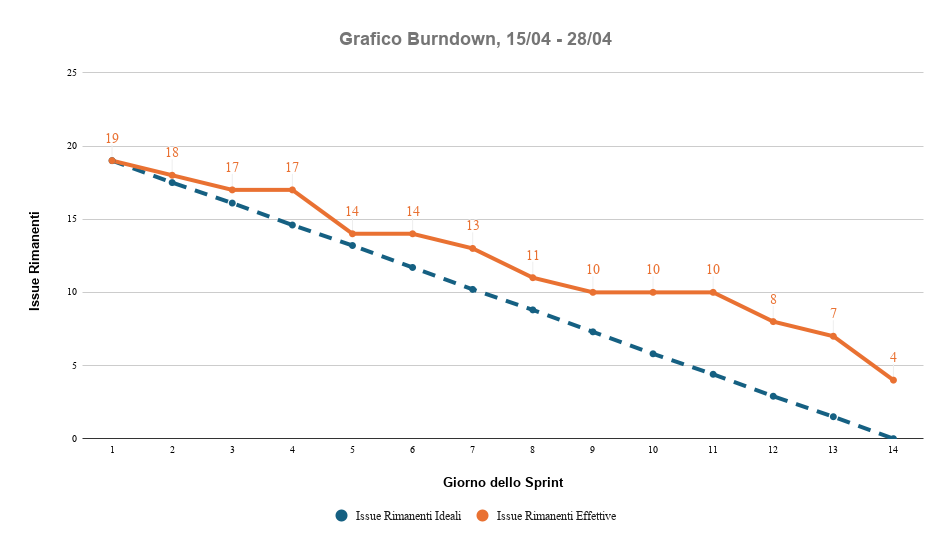
\includegraphics[width=0.9\textwidth]{grafici/burndown_sprint2.png}
    \caption{\textit{Grafico Burndown} - \textit{Sprint} 2}
    \label{fig:burndown-sprint2}
\end{figure}

\paragraph{Analisi dei rischi occorsi}
Durante lo svolgimento del secondo \textit{Sprint}, l'applicazione delle misure di mitigazione per il rischio \textbf{RO1 (Genericità dei task)} ha prodotto esiti positivi, tuttavia l'aumento della complessità gestionale ha fatto emergere una nuova criticità:

\begin{itemize}
    \item \textbf{Difficoltà nel coordinamento dei ruoli (RO2):} Con l'introduzione di una scomposizione più fine delle attività in \textit{Issue} atomiche, è emersa una difficoltà iniziale nel coordinare il lavoro sincrono tra i diversi ruoli.
\item \textbf{Mitigazione:} Per risolvere tempestivamente l'intoppo, il gruppo ha deciso di avere una comunicazione più frequente tramite \textit{\glo{WhatsApp}{whatsapp}} e \textit{\glo{Discord}{discord}}.
Questa misura ha permesso di ridistribuire il carico di lavoro in tempo reale, garantendo agli \textbf{Analisti} le linee guida necessarie per procedere senza ulteriori blocchi.
\item \textbf{\textit{Issue} non chiuse:} Non siamo riusciti a chiudere tutte le \textit{Issue} aperte a cause delle difficoltà che abbiamo incontrato nella gestione dei ruoli e delle proprie ore(come si vede nel grafico \textit{Burndown Chart}).
\end{itemize}

\paragraph{\textit{Retrospettiva}}
Il bilancio dello \textit{Sprint} 2 mostra un netto miglioramento qualitativo nel metodo di lavoro e una gestione più consapevole delle risorse economiche e temporali rispetto al periodo precedente.
\paragraph{Cosa ha funzionato:}
\begin{itemize}
    \item \textbf{Efficacia della granularità:} La scomposizione delle macro-attività in \textit{Issue} atomiche ha permesso un monitoraggio molto più preciso;
lo stato di avanzamento dell'\textbf{Analisi dei Requisiti} è risultato chiaro a tutti i membri del gruppo in ogni momento.
\item \textbf{Monitoraggio Data-driven:} L'adozione dei \textit{Burndown Chart} è stata fondamentale per identificare precocemente un rallentamento a metà \textit{Sprint}, consentendo al \textbf{Responsabile} di intervenire proattivamente prima che la scadenza diventasse critica.
\end{itemize}

\paragraph{Migliorie per lo \textit{Sprint} 3:}
\begin{itemize}
    \item \textbf{Gestione delle dipendenze:} Nonostante l'atomicità dei task, è emersa la necessità di definire meglio l'ordine di esecuzione (propedeuticità) quando un'attività dipende da un'altra (es. la fase di verifica subordinata al completamento della stesura).
\item \textbf{Standardizzazione dei documenti:} Per ottimizzare i tempi di formattazione \textit{\glo{LaTeX}{latex}}, che sono risultati superiori al previsto, il team ha deciso di sviluppare dei template pre-impostati per ogni tipologia di documento, velocizzando così la futura stesura tecnica.
\end{itemize}

\subsubsection{\textit{Sprint} 3: 28/04/2026 - 12/05/2026}

\paragraph{Obiettivi e attività}

Le attività previste per il terzo \textit{Sprint} sono le seguenti:

\begin{itemize}
\item
    iniziare il Glossario;
\item
  convertire i documenti in sviluppo (\textbf{Analisi dei Requisiti}, \textbf{Norme di Progetto} e \textbf{Piano di Progetto}) in \textit{LaTeX};
\item
  \textbf{Analisi dei Requisiti}: continuare gli \textit{Use Case} dei 3
  agenti da sviluppare;
\item
  \textbf{Norme di Progetto}: continuare i processi primari e processi
  organizzativi;
\item
  \textbf{Piano di Progetto}: stesura Pianificazione, scrivere \textit{Consuntivo} \textit{Sprint} 2 e \textit{Preventivo} \textit{Sprint} 3.
\end{itemize}


\paragraph{\textit{Preventivo} orario ed economico}

I ruoli assegnati sono: \textbf{Responsabile}, \textbf{Amministratore}, \textbf{Analista} e \textbf{Verificatore}.
\begin{table}[H]
    \centering
    \renewcommand{\arraystretch}{1.3}
    \begin{tabularx}{0.9\textwidth}{|X|c|c|c|c|c|c|c|}
        \hline
        \textbf{\textit{Sprint} 3} & \textbf{RE} & \textbf{AM} & \textbf{AN} &
        \textbf{PG} & \textbf{PR} & \textbf{VE} & \textbf{Totale} \\ \hline
        Andrea Fistarol & & 5 & & & & &\textbf{5} \\ \hline
        Dario Pirrone & & & & & & 3 &\textbf{3} \\ \hline
        Edoardo Granziero & & 4 & & & & &\textbf{4} \\ \hline
        Marco Barbiero & & & 3 & & & &\textbf{3} \\ \hline
        Samuele Bertin & 5 & & & & & &\textbf{5} \\ \hline
        Sara Ristovic & & & 8 & & & &\textbf{8} \\ \hline
        \textbf{Ore totali per ruolo} & \textbf{5} & \textbf{9} &
        \textbf{11} & \textbf{0} & \textbf{0} & \textbf{3} & \textbf{28}\\ \hline
 
    \end{tabularx}
    \caption{Preventivo orario - \textit{Sprint} 3}
\end{table}

Le risorse economiche previste per lo \textit{Sprint} sono:

\begin{table}[H]
    \centering
    \renewcommand{\arraystretch}{1.3}
    \begin{tabularx}{0.9\textwidth}{|X|c|c|c|c|c|c|c|}
        \hline
        \textbf{\textit{Sprint} 3} & \textbf{RE} & \textbf{AM} & \textbf{AN} &
        \textbf{PG} & \textbf{PR} & \textbf{VE} & \textbf{Totale} \\ \hline
        \textbf{Costo orario} & \EUR{30} & \EUR{20} & \EUR{25} & \EUR{25} & \EUR{15}
        & \EUR{15} & 
/ \\ \hline
        \textbf{Costo totale} & \EUR{150} & \EUR{180} & \EUR{275} & \EUR{0} & \EUR{0} & 
        \EUR{45} & \textbf{\EUR{650}} \\ \hline
    \end{tabularx}
    \caption{Preventivo economico - \textit{Sprint} 3}
\end{table}

\paragraph{\textit{Consuntivo}}

È risultato un consumo orario correttamente preventivato inizialmente per tutti i ruoli.
\begin{table}[H]
    \centering
    \renewcommand{\arraystretch}{1.3}
    \begin{tabularx}{0.9\textwidth}{|X|c|c|c|c|c|c|c|}
        \hline
        \textbf{\textit{Sprint} 3} & \textbf{RE} & \textbf{AM} & \textbf{AN} &
        \textbf{PG} & \textbf{PR} & \textbf{VE} & \textbf{Totale} \\ \hline
        Andrea Fistarol & & 5 & & & & &\textbf{5} \\ \hline
        Dario Pirrone & & & & & & 3 &\textbf{3} \\ \hline
        Edoardo Granziero & & 4 & & & & &\textbf{4} \\ \hline
        Marco Barbiero & & & 3 & & & &\textbf{3} \\ \hline
        Samuele Bertin & 5 & & & & & &\textbf{5} \\ \hline
        Sara Ristovic & & & 8 & & & &\textbf{8} \\ \hline
        \textbf{Ore totali per ruolo} & \textbf{5} & \textbf{9} &
        \textbf{11} & \textbf{0} & \textbf{0} & \textbf{3} & \textbf{28}\\ \hline
 
    \end{tabularx}
    \caption{Consuntivo orario - \textit{Sprint} 3}
\end{table}

Le risorse economiche utilizzate durante lo \textit{Sprint} sono:

\begin{table}[H]
    \centerline{
        \centering
        \renewcommand{\arraystretch}{1.3}
        \begin{tabularx}{1.09\textwidth}{|X|c|c|c|c|c|c|c|}
            \hline
            \textbf{\textit{Sprint} 3} & \textbf{RE} & \textbf{AM} & \textbf{AN} &
            \textbf{PG} & \textbf{PR} & \textbf{VE} & \textbf{Totale} \\ \hline
  
            \textbf{Costo orario} & \EUR{30} & \EUR{20} & \EUR{25} & \EUR{25} & \EUR{15}
            & \EUR{15} & / \\ \hline
            \textbf{Costo totale} & \EUR{150} & \EUR{180} & \EUR{275} & \EUR{0} & \EUR{0} & 
            \EUR{45} & \textbf{\EUR{650}} \\ \hline
            \textbf{Saldo a fine \textit{Sprint}} & \textbf{\EUR{1.320}} & \textbf{\EUR{640}} & 
\textbf{\EUR{950}} 
            & \textbf{\EUR{2.700}} & \textbf{\EUR{2.070}} & \textbf{\EUR{2.130}} & \textbf{\EUR{9.810}}\\ \hline
        \end{tabularx}
    }
    \caption{\textit{Consuntivo} economico - \textit{Sprint} 3}
\end{table}

\begin{figure}[H]
    \centering
    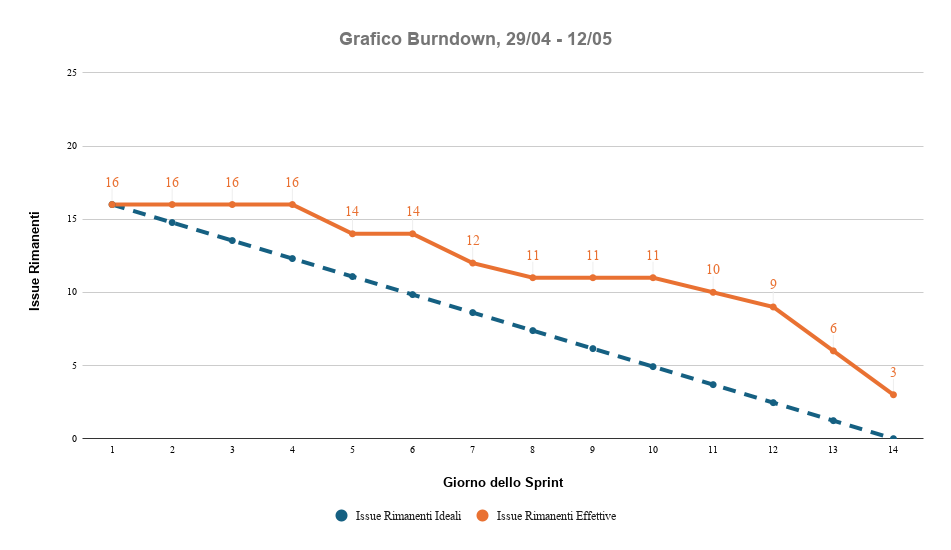
\includegraphics[width=0.9\textwidth]{grafici/burndown_sprint3.png}
    \caption{\textit{Grafico Burndown} - \textit{Sprint} 3}
    \label{fig:burndown-sprint3}
\end{figure}

\paragraph{Analisi dei rischi occorsi}

Durante lo svolgimento del terzo \textit{Sprint} è riemersa una criticità legata alla pianificazione (\textbf{RO1 - Scarsa Pianificazione}).
La divisione delle \textit{Issue} non si è rivelata sufficientemente granulare: avere task troppo ampi non ci ha permesso di tracciare i progressi nel migliore dei modi.
Questo ha reso la lettura del \textit{Burndown Chart} poco indicativa dello stato reale dei lavori e, soprattutto, ha generato un collo di bottiglia, impedendoci di chiudere definitivamente diverse attività prima della fine dello \textit{Sprint}.
\paragraph{\textit{Retrospettiva}}

Il terzo \textit{Sprint} ha consolidato l'infrastruttura documentale, ma ha evidenziato evidenti limiti operativi nella gestione e chiusura dei task.

\textbf{Cosa ha funzionato:}
\begin{itemize}
    \item \textbf{Standardizzazione in \textit{LaTeX}:} L'adozione dei nuovi template in \textit{LaTeX} ha reso il lavoro documentale molto più ordinato.
L'omogeneità stilistica e la struttura preimpostata hanno facilitato notevolmente la stesura, ripagando l'investimento di tempo fatto nello \textit{Sprint} precedente e rendendo i documenti molto più manutenibili.
\end{itemize}

\textbf{Cosa migliorare per lo \textit{Sprint} 4:}
\begin{itemize}
    \item \textbf{Scomposizione atomica e chiusura delle \textit{Issue}:} A causa della scarsa granularità, molte attività previste non sono arrivate allo stato di "Done" e sono slittate allo \textit{Sprint} successivo.
Per lo \textit{Sprint} 4, il team si impegnerà a spezzare i task in unità di lavoro molto più piccole e indipendenti, per garantirne la chiusura tempestiva, evitare lo \emph{spillover} tra \textit{Sprint} e permettere un tracciamento continuo e reale dei progressi.
\end{itemize}

\subsubsection{\textit{Sprint} 4: 12/05/2026 - 26/05/2026}

\paragraph{Obiettivi e attività}

Le attività previste per il quarto \textit{Sprint} sono le seguenti:

\begin{itemize}
    \item \textbf{Analisi dei Requisiti}: completamento degli \textit{Use Case} per gli agenti \textit{README}, \textit{Changelog} e \textit{OWASP}, stesura della sezione di Tracciamento e completamento della tabella dei Requisiti;
\item \textbf{Piano di Qualifica}: stesura dei capitoli 2.1, 2.2 e 2.3;
\item \textbf{Norme di Progetto}: stesura del capitolo relativo allo sviluppo;
\item \emph{Gestione documentale e \textit{Repository}:} aggiornamento del Glossario con introduzione di nuovi termini e creazione dei collegamenti tra documenti e glossario, sistemazione della struttura delle cartelle \textit{\glo{GitHub}{github}} per i file \texttt{.tex} e sistemazione dei template dei documenti;
\end{itemize}

\paragraph{\textit{Preventivo} orario ed economico}

I ruoli assegnati sono: \textbf{Responsabile}, \textbf{Amministratore}, \textbf{Analista} e \textbf{Verificatore}.
\begin{table}[H]
    \centering
    \renewcommand{\arraystretch}{1.3}
    \begin{tabularx}{0.9\textwidth}{|X|c|c|c|c|c|c|c|}
        \hline
        \textbf{\textit{Sprint} 4} & \textbf{RE} & \textbf{AM} & \textbf{AN} &
        \textbf{PG} & \textbf{PR} & \textbf{VE} & \textbf{Totale} \\ \hline
        Andrea Fistarol & & & 4 & & & & \textbf{4} \\ \hline
        Dario Pirrone & & 5 & & & & & \textbf{5} \\ \hline
        Edoardo Granziero & 4 & & & & & & \textbf{4} \\ \hline
        Marco Barbiero & & & 5 & & & & \textbf{5} \\ \hline
        Samuele Bertin & & & & & & 3 & \textbf{3} \\ \hline
        Sara Ristovic & & & 6 & & & & \textbf{6} \\ \hline
        \textbf{Ore totali per ruolo} & \textbf{4} & \textbf{5} &
        \textbf{15} & \textbf{0} & \textbf{0} & \textbf{3} & \textbf{27}\\ \hline
    \end{tabularx}
    \caption{Preventivo orario - \textit{Sprint} 4}
\end{table}

Le risorse economiche previste per lo \textit{Sprint} sono:

\begin{table}[H]
    \centering
    \renewcommand{\arraystretch}{1.3}
    \begin{tabularx}{0.9\textwidth}{|X|c|c|c|c|c|c|c|}
        \hline
        \textbf{\textit{Sprint} 4} & \textbf{RE} & \textbf{AM} & \textbf{AN} &
        \textbf{PG} & \textbf{PR} & \textbf{VE} & \textbf{Totale} \\ \hline
        \textbf{Costo orario} & \EUR{30} & \EUR{20} & \EUR{25} & \EUR{25} & \EUR{15}
     
        & \EUR{15} & / \\ \hline
        \textbf{Costo totale} & \EUR{120} & \EUR{100} & \EUR{375} & \EUR{0} & \EUR{0} & \EUR{45} & \textbf{\EUR{640}} \\ \hline
    \end{tabularx}
    \caption{Preventivo economico - \textit{Sprint} 4}
\end{table}

\paragraph{\textit{Consuntivo}}

È risultato un consumo orario leggermente superiore al quanto  preventivato inizialmente.

\begin{table}[H]
    \centering
    \renewcommand{\arraystretch}{1.3}
    \begin{tabularx}{0.9\textwidth}{|X|c|c|c|c|c|c|c|}
        \hline
        \textbf{\textit{Sprint} 4} & \textbf{RE} & \textbf{AM} & \textbf{AN} &
        \textbf{PG} & \textbf{PR} & \textbf{VE} & \textbf{Totale} \\ \hline
        Andrea Fistarol & & & 4 & & & &\textbf{4} \\ \hline
        Dario Pirrone & & 4 (-1) & & & & &\textbf{4} \\ \hline
        Edoardo Granziero & 4 & & & & & &\textbf{4} \\ \hline
        Marco Barbiero & & & 5 & & & &\textbf{5} \\ \hline
        Samuele Bertin & & & & & & 4 (+1) &\textbf{4} \\ \hline
        Sara Ristovic & & & 8 (+2) & & & &\textbf{8} \\ \hline
        \textbf{Ore totali per ruolo} & \textbf{4} & \textbf{4} &
        \textbf{17} & \textbf{0} & \textbf{0} & \textbf{4} & \textbf{29}\\ \hline
 
    \end{tabularx}
    \caption{Consuntivo orario - \textit{Sprint} 4}
\end{table}

Le risorse economiche utilizzate durante lo \textit{Sprint} sono:

\begin{table}[H]
    \centerline{
        \centering
        \renewcommand{\arraystretch}{1.3}
        \begin{tabularx}{1.09\textwidth}{|X|c|c|c|c|c|c|c|}
            \hline
            \textbf{\textit{Sprint} 4} & \textbf{RE} & \textbf{AM} & \textbf{AN} &
            \textbf{PG} & \textbf{PR} & \textbf{VE} & \textbf{Totale} \\ \hline
  
            \textbf{Costo orario} & \EUR{30} & \EUR{20} & \EUR{25} & \EUR{25} & \EUR{15}
            & \EUR{15} & / \\ \hline
            \textbf{Costo totale} & \EUR{120} & \EUR{80} & \EUR{425} & \EUR{0} & \EUR{0} & 
            \EUR{60} & \textbf{\EUR{685}} \\ \hline
            \textbf{Saldo a fine \textit{Sprint}} & \textbf{\EUR{1.200}} & \textbf{\EUR{560}} & \textbf{\EUR{525}} & \textbf{\EUR{2.700}} & \textbf{\EUR{2.070}} & \textbf{\EUR{2.070}} & \textbf{\EUR{9.125}}\\ \hline
        \end{tabularx}
    }
    \caption{\textit{Consuntivo} economico - \textit{Sprint} 4}
\end{table}

\begin{figure}[H]
    \centering
    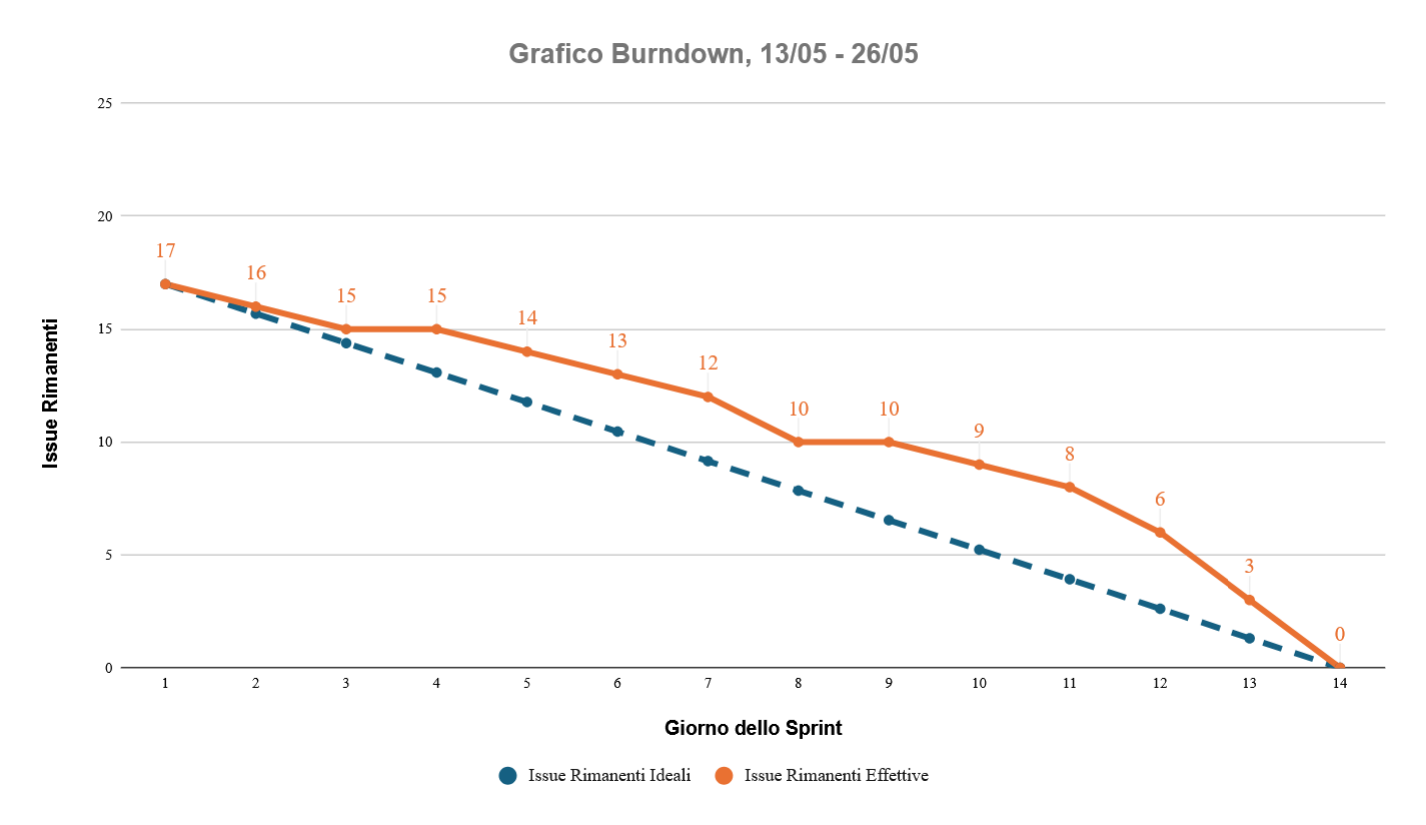
\includegraphics[width=0.9\textwidth]{grafici/burndown_sprint4.png}
    \caption{\textit{Grafico Burndown} - \textit{Sprint} 4}
    \label{fig:burndown-sprint4}
\end{figure}

\paragraph{Analisi dei rischi occorsi}
Durante lo \textit{Sprint 4} si è manifestato il rischio relativo alla comunicazione inefficiente con il \textbf{Proponente}, identificato come RO3. \\
A causa di tale difficoltà comunicativa, è stato necessario attendere più del previsto per fissare un incontro con il \textbf{Proponente}, finalizzato alla discussione dell'\textbf{Analisi dei Requisiti} e alla ricezione del primo riscontro significativo sul documento. Ciò ha causato un ritardo nello svolgimento del progetto e la necessità di rivalutare alcune scadenze interne.

\paragraph{\textit{Retrospettiva}}
Nonostante il rischio occorso, è stato comunque effettuato un buon avanzamento nella stesura di tutti i documenti previsti finora.

\paragraph{Cosa ha funzionato:}
\begin{itemize}
    \item \textbf{\textit{issue} "non assegnate":} Questo tipo di compito è stato introdotto per garantire maggiore flessibilità ai membri del gruppo. Qualora un membro avesse completato le proprie \textit{issue} assegnate prima della fine dello \textit{Sprint} e avesse avuto ancora tempo a disposizione, poteva assegnarsi una delle \textit{issue} inizialmente indicate come non assegnate.  Tutte le \textit{issue} di questo tipo sono state completate, contribuendo ad aumentare la produttività del gruppo.
    \item \textbf{comunicazione interna sullo stato di avanzamento a metà dello \textit{Sprint}:} Il gruppo ha ritenuto necessario comunicare più spesso lo stato di avanzamento del lavoro di ogni membro durante lo \textit{Sprint}, poiché gli \textit{Sprint} durano due settimane e si vuole promuovere un lavoro continuo. È stato concluso che questa comunicazione asincrona sullo stato di avanzamento ha aiutato i membri a lavorare meglio, dato che lo \textit{Sprint} si è concluso con tutte le \textit{issue} chiuse, risolvendo una criticità emersa nello \textit{Sprint} precedente.
\end{itemize}

\paragraph{Migliorie per lo \textit{Sprint} 5:}
\begin{itemize}
    \item \textbf{mitigazioni per il rischio riscontrato:} In futuro, durante la comunicazione tramite messaggi su \textit{Slack}, il gruppo taggherà sempre la persona esterna a cui si rivolge, poiché questa pratica si è dimostrata utile. Inoltre, le richieste importanti da parte del gruppo verranno formulate anche in forma scritta e non solamente oralmente durante gli incontri esterni.
    \item \textbf{incontro interno a metà dello \textit{Sprint}:} 
    Si è deciso di svolgere questo incontro per monitorare meglio l’avanzamento dei compiti dello \textit{Sprint}, pratica che si è rivelata molto utile nello \textit{Sprint} precedente, e per concordare più aspetti importanti.
\end{itemize}


\subsubsection{\textit{Sprint} 5: 26/05/2026 - 09/06/2026}

\paragraph{Obiettivi e attività}

Le attività previste per il quinto \textit{Sprint}, ordinate in base alla priorità, sono le seguenti:

\begin{itemize}
    \item ricevere riscontro sull'\textbf{Analisi dei Requisiti}, effettuare le modifiche necessarie e chiudere la stesura del documento
    \item decidere le tecnologie per l'implementazione del \textit{PoC}
    \item avanzare nella stesura del \textbf{Piano di Qualifica}
    \item se possibile, iniziare la realizzazione del \textit{PoC}
\end{itemize}

\paragraph{\textit{Preventivo} orario ed economico}

I ruoli assegnati sono: \textbf{Responsabile}, \textbf{Amministratore}, \textbf{Analista}, \textbf{\glo{Progettista}{progettista}} e \textbf{Verificatore}.
\begin{table}[H]
    \centering
    \renewcommand{\arraystretch}{1.3}
    \begin{tabularx}{0.9\textwidth}{|X|c|c|c|c|c|c|c|}
        \hline
        \textbf{\textit{Sprint} 5} & \textbf{RE} & \textbf{AM} & \textbf{AN} &
        \textbf{PG} & \textbf{PR} & \textbf{VE} & \textbf{Totale} \\ \hline
        Andrea Fistarol & & & 5 & & & & \textbf{5} \\ \hline
        Dario Pirrone & & & 7 & & & & \textbf{7} \\ \hline
        Edoardo Granziero & & & & & & 3 & \textbf{3} \\ \hline
        Marco Barbiero & & & & 8 & & & \textbf{8} \\ \hline
        Samuele Bertin & & 5 & & & & & \textbf{5} \\ \hline
        Sara Ristovic & 5 & & & & & & \textbf{5} \\ \hline
        \textbf{Ore totali per ruolo} & \textbf{5} & \textbf{5} &
        \textbf{12} & \textbf{8} & \textbf{0} & \textbf{3} & \textbf{33}\\ \hline
    \end{tabularx}
    \caption{Preventivo orario - \textit{Sprint} 5}
\end{table}

Le risorse economiche previste per lo \textit{Sprint} sono:

\begin{table}[H]
    \centering
    \renewcommand{\arraystretch}{1.3}
    \begin{tabularx}{0.9\textwidth}{|X|c|c|c|c|c|c|c|}
        \hline
        \textbf{\textit{Sprint} 4} & \textbf{RE} & \textbf{AM} & \textbf{AN} &
        \textbf{PG} & \textbf{PR} & \textbf{VE} & \textbf{Totale} \\ \hline
        \textbf{Costo orario} & \EUR{30} & \EUR{20} & \EUR{25} & \EUR{25} & \EUR{15}
     
        & \EUR{15} & / \\ \hline
        \textbf{Costo totale} & \EUR{150} & \EUR{100} & \EUR{300} & \EUR{200} & \EUR{0} & \EUR{45} & \textbf{\EUR{795}} \\ \hline
    \end{tabularx}
    \caption{Preventivo economico - \textit{Sprint} 5}
\end{table}

\paragraph{\textit{Consuntivo}}

È risultato un consumo orario leggermente superiore al quanto  preventivato inizialmente.

\begin{table}[H]
    \centering
    \renewcommand{\arraystretch}{1.3}
    \begin{tabularx}{0.9\textwidth}{|X|c|c|c|c|c|c|c|}
        \hline
        \textbf{\textit{Sprint} 5} & \textbf{RE} & \textbf{AM} & \textbf{AN} &
        \textbf{PG} & \textbf{PR} & \textbf{VE} & \textbf{Totale} \\ \hline
        Andrea Fistarol & & & 5 & & & & \textbf{5} \\ \hline
        Dario Pirrone & & & 8 (+1) & & & & \textbf{8} \\ \hline
        Edoardo Granziero & & & & & & 4 (+1) & \textbf{4} \\ \hline
        Marco Barbiero & & & & 8 & & & \textbf{8} \\ \hline
        Samuele Bertin & & 4 (-1) & & & & & \textbf{4} \\ \hline
        Sara Ristovic & 5 & & & & & & \textbf{5} \\ \hline
        \textbf{Ore totali per ruolo} & \textbf{5} & \textbf{4} &
        \textbf{13} & \textbf{8} & \textbf{0} & \textbf{4} & \textbf{34}\\ \hline
 
    \end{tabularx}
    \caption{Consuntivo orario - \textit{Sprint} 5}
\end{table}

Le risorse economiche utilizzate durante lo \textit{Sprint} sono:

\begin{table}[H]
    \centerline{
        \centering
        \renewcommand{\arraystretch}{1.3}
        \begin{tabularx}{1.09\textwidth}{|X|c|c|c|c|c|c|c|}
            \hline
            \textbf{\textit{Sprint} 5} & \textbf{RE} & \textbf{AM} & \textbf{AN} &
            \textbf{PG} & \textbf{PR} & \textbf{VE} & \textbf{Totale} \\ \hline
  
            \textbf{Costo orario} & \EUR{30} & \EUR{20} & \EUR{25} & \EUR{25} & \EUR{15}
            & \EUR{15} & / \\ \hline
            \textbf{Costo totale} & \EUR{150} & \EUR{80} & \EUR{325} & \EUR{200} & \EUR{0} & 
            \EUR{60} & \textbf{\EUR{815}} \\ \hline
            \textbf{Saldo a fine \textit{Sprint}} & \textbf{\EUR{1.050}} & \textbf{\EUR{480}} & \textbf{\EUR{200}} & \textbf{\EUR{2.500}} & \textbf{\EUR{2.070}} & \textbf{\EUR{2.010}} & \textbf{\EUR{8.310}}\\ \hline
        \end{tabularx}
    }
    \caption{\textit{Consuntivo} economico - \textit{Sprint} 5}
\end{table}

\begin{figure}[H]
    \centering
    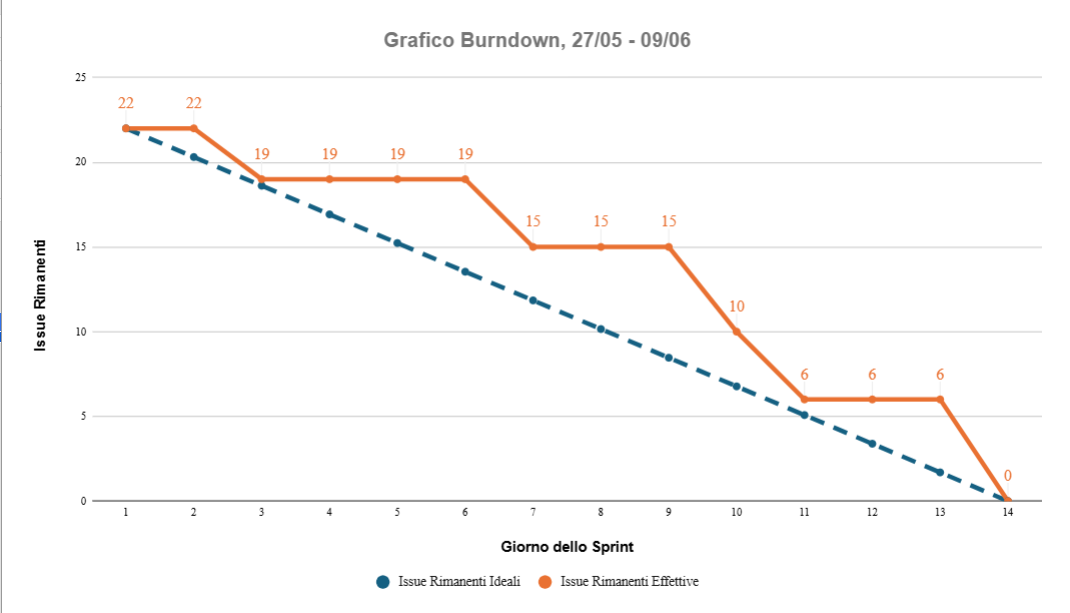
\includegraphics[width=0.9\textwidth]{grafici/burndown_sprint5.png}
    \caption{\textit{Grafico Burndown} - \textit{Sprint} 5}
    \label{fig:burndown-sprint5}
\end{figure}

\paragraph{Analisi dei rischi occorsi}
\begin{itemize}
     \item Durante lo \textit{Sprint} si è concretizzato il rischio di un disallineamento informativo con il \textbf{Proponente} riguardo l'architettura di partenza. L'assenza di un \textbf{orchestratore agenti} proprietario preesistente, contrariamente alle ipotesi preliminari, richiederà uno sforzo aggiuntivo.\\
     L'imprevisto ha causato un incremento del carico di lavoro e un rallentamento sulla tabella di marcia originaria.\\
\end{itemize}

\paragraph{Retrospettiva: cosa ha funzionato}
\begin{itemize}
    \item \textbf{Avvio tempestivo e strutturato del \textit{PoC}:} Nonostante l'imprevisto tecnico riscontrato con l'azienda, l'assegnazione mirata delle ore al ruolo di \textit{Progettista} ha permesso di definire con successo lo scheletro architetturale del \textit{Proof of Concept} e di completare una parte significativa del suo sviluppo funzionale.
    \item \textbf{Raffinamento proattivo dei requisiti:} Gli \textit{Analisti} hanno individuato le aree critiche dell'\textbf{Analisi dei Requisiti} e hanno avviato una sessione di correzione dei \textit{casi d'uso} e irrobustimento del tracciamento, preparandosi al colloquio di revisione con il Prof. Cardin.
\end{itemize}

\paragraph{Migliorie per lo Sprint 6}
\begin{itemize}
    \item \textbf{Parallelizzazione tra sviluppo del PoC e correzione documentale:} Sfruttando l'insieme delle tecnologie del \textit{PoC} ormai consolidato, si prevede di separare nettamente i flussi di lavoro nello \textit{Sprint} 6.
\end{itemize}

\subsubsection{\textit{Sprint} 6: 10/06/2026 - 23/06/2026}

\paragraph{Obiettivi e attività}

Le attività previste per il sesto \textit{Sprint}, ordinate in base alla priorità, sono le seguenti:

\begin{itemize}
    \item  verifica e correzione dell'\textbf{Analisi dei Requisiti} in preparzione del ricevimento con il Prof. Cardin
    \item Andare avanti con il \textit{PoC}
    \item verifica e modifica della documentazione per l'\textbf{RTB}.
\end{itemize}

\paragraph{\textit{Preventivo} orario ed economico}

I ruoli assegnati sono: \textbf{Responsabile}, \textbf{Amministratore}, \textbf{Analista}, \textbf{Progettista} e \textbf{Verificatore}.
\begin{table}[H]
    \centering
    \renewcommand{\arraystretch}{1.3}
    \begin{tabularx}{0.9\textwidth}{|X|c|c|c|c|c|c|c|}
        \hline
        \textbf{\textit{Sprint} 6} & \textbf{RE} & \textbf{AM} & \textbf{AN} &
        \textbf{PG} & \textbf{PR} & \textbf{VE} & \textbf{Totale} \\ \hline
        Andrea Fistarol & & & & & 1 & &\textbf{1} \\ \hline
        Dario Pirrone & & & 2 & & & & \textbf{2} \\ \hline
        Edoardo Granziero & & 1 & & & & & \textbf{1} \\ \hline
        Marco Barbiero & & & & & 1 & & \textbf{1} \\ \hline
        Samuele Bertin & 2 & & & & & & \textbf{2} \\ \hline
        Sara Ristovic & & & & & & 1 & \textbf{1} \\ \hline
        \textbf{Ore totali per ruolo} & \textbf{2} & \textbf{1} &
        \textbf{2} & \textbf{0} & \textbf{2} & \textbf{1} & \textbf{8}\\ \hline
    \end{tabularx}
    \caption{Preventivo orario - \textit{Sprint} 6}
\end{table}

Le risorse economiche previste per lo \textit{Sprint} sono:

\begin{table}[H]
    \centering
    \renewcommand{\arraystretch}{1.3}
    \begin{tabularx}{0.9\textwidth}{|X|c|c|c|c|c|c|c|}
        \hline
        \textbf{\textit{Sprint} 6} & \textbf{RE} & \textbf{AM} & \textbf{AN} &
        \textbf{PG} & \textbf{PR} & \textbf{VE} & \textbf{Totale} \\ \hline
        \textbf{Costo orario} & \EUR{30} & \EUR{20} & \EUR{25} & \EUR{25} & \EUR{15}
     
        & \EUR{15} & / \\ \hline
        \textbf{Costo totale} & \EUR{} & \EUR{} & \EUR{} & \EUR{} & \EUR{} & \EUR{} & \textbf{\EUR{}} \\ \hline
    \end{tabularx}
    \caption{Preventivo economico - \textit{Sprint} 6}
\end{table}

\paragraph{\textit{Consuntivo}}

È risultato un consumo orario correttamente preventivato inizialmente.

\begin{table}[H]
    \centering
    \renewcommand{\arraystretch}{1.3}
    \begin{tabularx}{0.9\textwidth}{|X|c|c|c|c|c|c|c|}
        \hline
        \textbf{\textit{Sprint} 6} & \textbf{RE} & \textbf{AM} & \textbf{AN} &
        \textbf{PG} & \textbf{PR} & \textbf{VE} & \textbf{Totale} \\ \hline
        Andrea Fistarol & & & & & 1 & & \textbf{1} \\ \hline
        Dario Pirrone & & & 2 & & & & \textbf{2} \\ \hline
        Edoardo Granziero & & 1 & & & & & \textbf{1} \\ \hline
        Marco Barbiero & & & & & 1 & & \textbf{1} \\ \hline
        Samuele Bertin & 2 & & & & & & \textbf{2} \\ \hline
        Sara Ristovic & & & & & & 1 & \textbf{1} \\ \hline
        \textbf{Ore totali per ruolo} & \textbf{2} & \textbf{1} &
        \textbf{2} & \textbf{0} & \textbf{2} & \textbf{1} & \textbf{8}\\ \hline
 
    \end{tabularx}
    \caption{Consuntivo orario - \textit{Sprint} 6}
\end{table}

Le risorse economiche utilizzate durante lo \textit{Sprint} sono:

\begin{table}[H]
    \centerline{
        \centering
        \renewcommand{\arraystretch}{1.3}
        \begin{tabularx}{1.09\textwidth}{|X|c|c|c|c|c|c|c|}
            \hline
            \textbf{\textit{Sprint} 6} & \textbf{RE} & \textbf{AM} & \textbf{AN} &
            \textbf{PG} & \textbf{PR} & \textbf{VE} & \textbf{Totale} \\ \hline
  
            \textbf{Costo orario} & \EUR{30} & \EUR{20} & \EUR{25} & \EUR{25} & \EUR{15}
            & \EUR{15} & / \\ \hline
            \textbf{Costo totale} & \EUR{60} & \EUR{20} & \EUR{50} & \EUR{0} & \EUR{30} & 
            \EUR{15} & \textbf{\EUR{175}} \\ \hline
            \textbf{Saldo a fine \textit{Sprint}} & \textbf{\EUR{990}} & \textbf{\EUR{460}} & \textbf{\EUR{150}} & \textbf{\EUR{2.500}} & \textbf{\EUR{2.040}} & \textbf{\EUR{1.995}} & \textbf{\EUR{8.135}}\\ \hline
        \end{tabularx}
    }
    \caption{\textit{Consuntivo} economico - \textit{Sprint} 6}
\end{table}

\paragraph{Analisi dei rischi occorsi}
\begin{itemize}
     \item Durante lo \textit{Sprint} 6 si è concretizzato il rischio legato alla concomitanza con la sessione d'esami estiva, che ha comportato una drastica e prevista riduzione della disponibilità oraria dei membri del team. Questo vincolo accademico personale ha rallentato temporaneamente il ritmo delle attività di sviluppo e stesura documentale.\\
\end{itemize}

\paragraph{Retrospettiva: cosa ha funzionato}
\begin{itemize}
    \item \textbf{Gestione del carico di lavoro minimo:} Nonostante le ore complessive dedicate al progetto siano state sensibilmente inferiori rispetto ai periodi precedenti, la pianificazione interna ha permesso di mantenere attivi i canali di comunicazione stabili e di non bloccare del tutto le attività propedeutiche.
    \item \textbf{Mantenimento dei requisiti di base:} Il team è riuscito a preservare l'integrità e il consolidamento di quanto sviluppato finora sul \textit{PoC} e sull'\textbf{Analisi dei Requisiti} durante gli Sprint passati, evitando regressioni o perdite di focus architetturale nonostante la ridotta operatività.
\end{itemize}

\paragraph{Migliorie per lo Sprint 7}
\begin{itemize}
    \item \textbf{Pianificazione di recupero e riallocazione del budget orario:} Con la conclusione della parte principale della sessione d'esami, lo \textit{Sprint} 7 dovrà prevedere una rimodulazione intensiva delle ore per recuperare il disavanzo dello sprint precedente, parallelizzando lo sviluppo pratico del \textit{PoC} (sfruttando le credenziali richieste) e la chiusura dei documenti.
    \item \textbf{Integrazione immediata degli asset esterni:} Al fine di ottimizzare i tempi di sviluppo rimasti, non appena verranno fornite le credenziali dell'ambiente cloud, si prevede l'istituzione di una sessione di sviluppo congiunta tra i programmatori per accelerare l'integrazione dell'orchestratore.
\end{itemize}

\subsubsection{\textit{Sprint} 7: 24/06/2026 - 07/07/2026}

\paragraph{Obiettivi e attività}

Le attività previste per il sesto \textit{Sprint}, ordinate in base alla priorità, sono le seguenti:

\begin{itemize}
    \item  verifica e correzione di tutta la documentazione in vista dell'\textbf{RTB}
    \item Sviluppo Frontend, Backend e Architettura del \textit{PoC}
    \item Perfezionamento dell'\textit{AdR}.
\end{itemize}

\paragraph{\textit{Preventivo} orario ed economico}

I ruoli assegnati sono: \textbf{Responsabile}, \textbf{Amministratore}, \textbf{Analista}, \textbf{Progettista} e \textbf{Verificatore}.
\begin{table}[H]
    \centering
    \renewcommand{\arraystretch}{1.3}
    \begin{tabularx}{0.9\textwidth}{|X|c|c|c|c|c|c|c|}
        \hline
        \textbf{\textit{Sprint} 7} & \textbf{RE} & \textbf{AM} & \textbf{AN} &
        \textbf{PG} & \textbf{PR} & \textbf{VE} & \textbf{Totale} \\ \hline
        Andrea Fistarol & & & & & & & \textbf{} \\ \hline
        Dario Pirrone & & & 2 & & & \textbf{} \\ \hline
        Edoardo Granziero & & & & & & & \textbf{} \\ \hline
        Marco Barbiero & & & & & & & \textbf{} \\ \hline
        Samuele Bertin & 2 & & & & & \textbf{} \\ \hline
        Sara Ristovic & & & & & & & \textbf{} \\ \hline
        \textbf{Ore totali per ruolo} & \textbf{0} & \textbf{0} &
        \textbf{0} & \textbf{0} & \textbf{0} & \textbf{0} & \textbf{0}\\ \hline
    \end{tabularx}
    \caption{Preventivo orario - \textit{Sprint} 7}
\end{table}

Le risorse economiche previste per lo \textit{Sprint} sono:

\begin{table}[H]
    \centering
    \renewcommand{\arraystretch}{1.3}
    \begin{tabularx}{0.9\textwidth}{|X|c|c|c|c|c|c|c|}
        \hline
        \textbf{\textit{Sprint} 7} & \textbf{RE} & \textbf{AM} & \textbf{AN} &
        \textbf{PG} & \textbf{PR} & \textbf{VE} & \textbf{Totale} \\ \hline
        \textbf{Costo orario} & \EUR{30} & \EUR{20} & \EUR{25} & \EUR{25} & \EUR{15}
     
        & \EUR{15} & / \\ \hline
        \textbf{Costo totale} & \EUR{} & \EUR{} & \EUR{} & \EUR{} & \EUR{} & \EUR{} & \textbf{\EUR{}} \\ \hline
    \end{tabularx}
    \caption{Preventivo economico - \textit{Sprint} 7}
\end{table}

\end{document}
